\documentclass[12pt]{article}
\usepackage[export]{adjustbox}
\usepackage[utf8]{inputenc}
\usepackage{graphicx}
\usepackage{caption}
\usepackage{subfig}
\usepackage{lipsum}
\usepackage{geometry}
\geometry{
 a4paper,
 total={170mm,257mm},
 left=20mm,
 top=20mm,
 }
%\usepackage{biblatex}
%\addbibresource{references.bib}



\title{COP290: Application for Moodle IIT Delhi}
\author{Aayan Kumar (2014CS10201) \\ Shreyan Gupta (2014CS10485) \\ Vaibhav Bhagee (2014CS50297) }

\begin{document}
\maketitle

The application provides an easy-to-use user interface to access the IIT Delhi Moodle on android platform. The application interacts with a locally deployed Web2Py through API calls and provides the relevant functionality to the user. 

\section{User Interface}

\begin{center}
\begin{tabular}{c c c}
     
\begin{minipage}[t]{.3\textwidth}
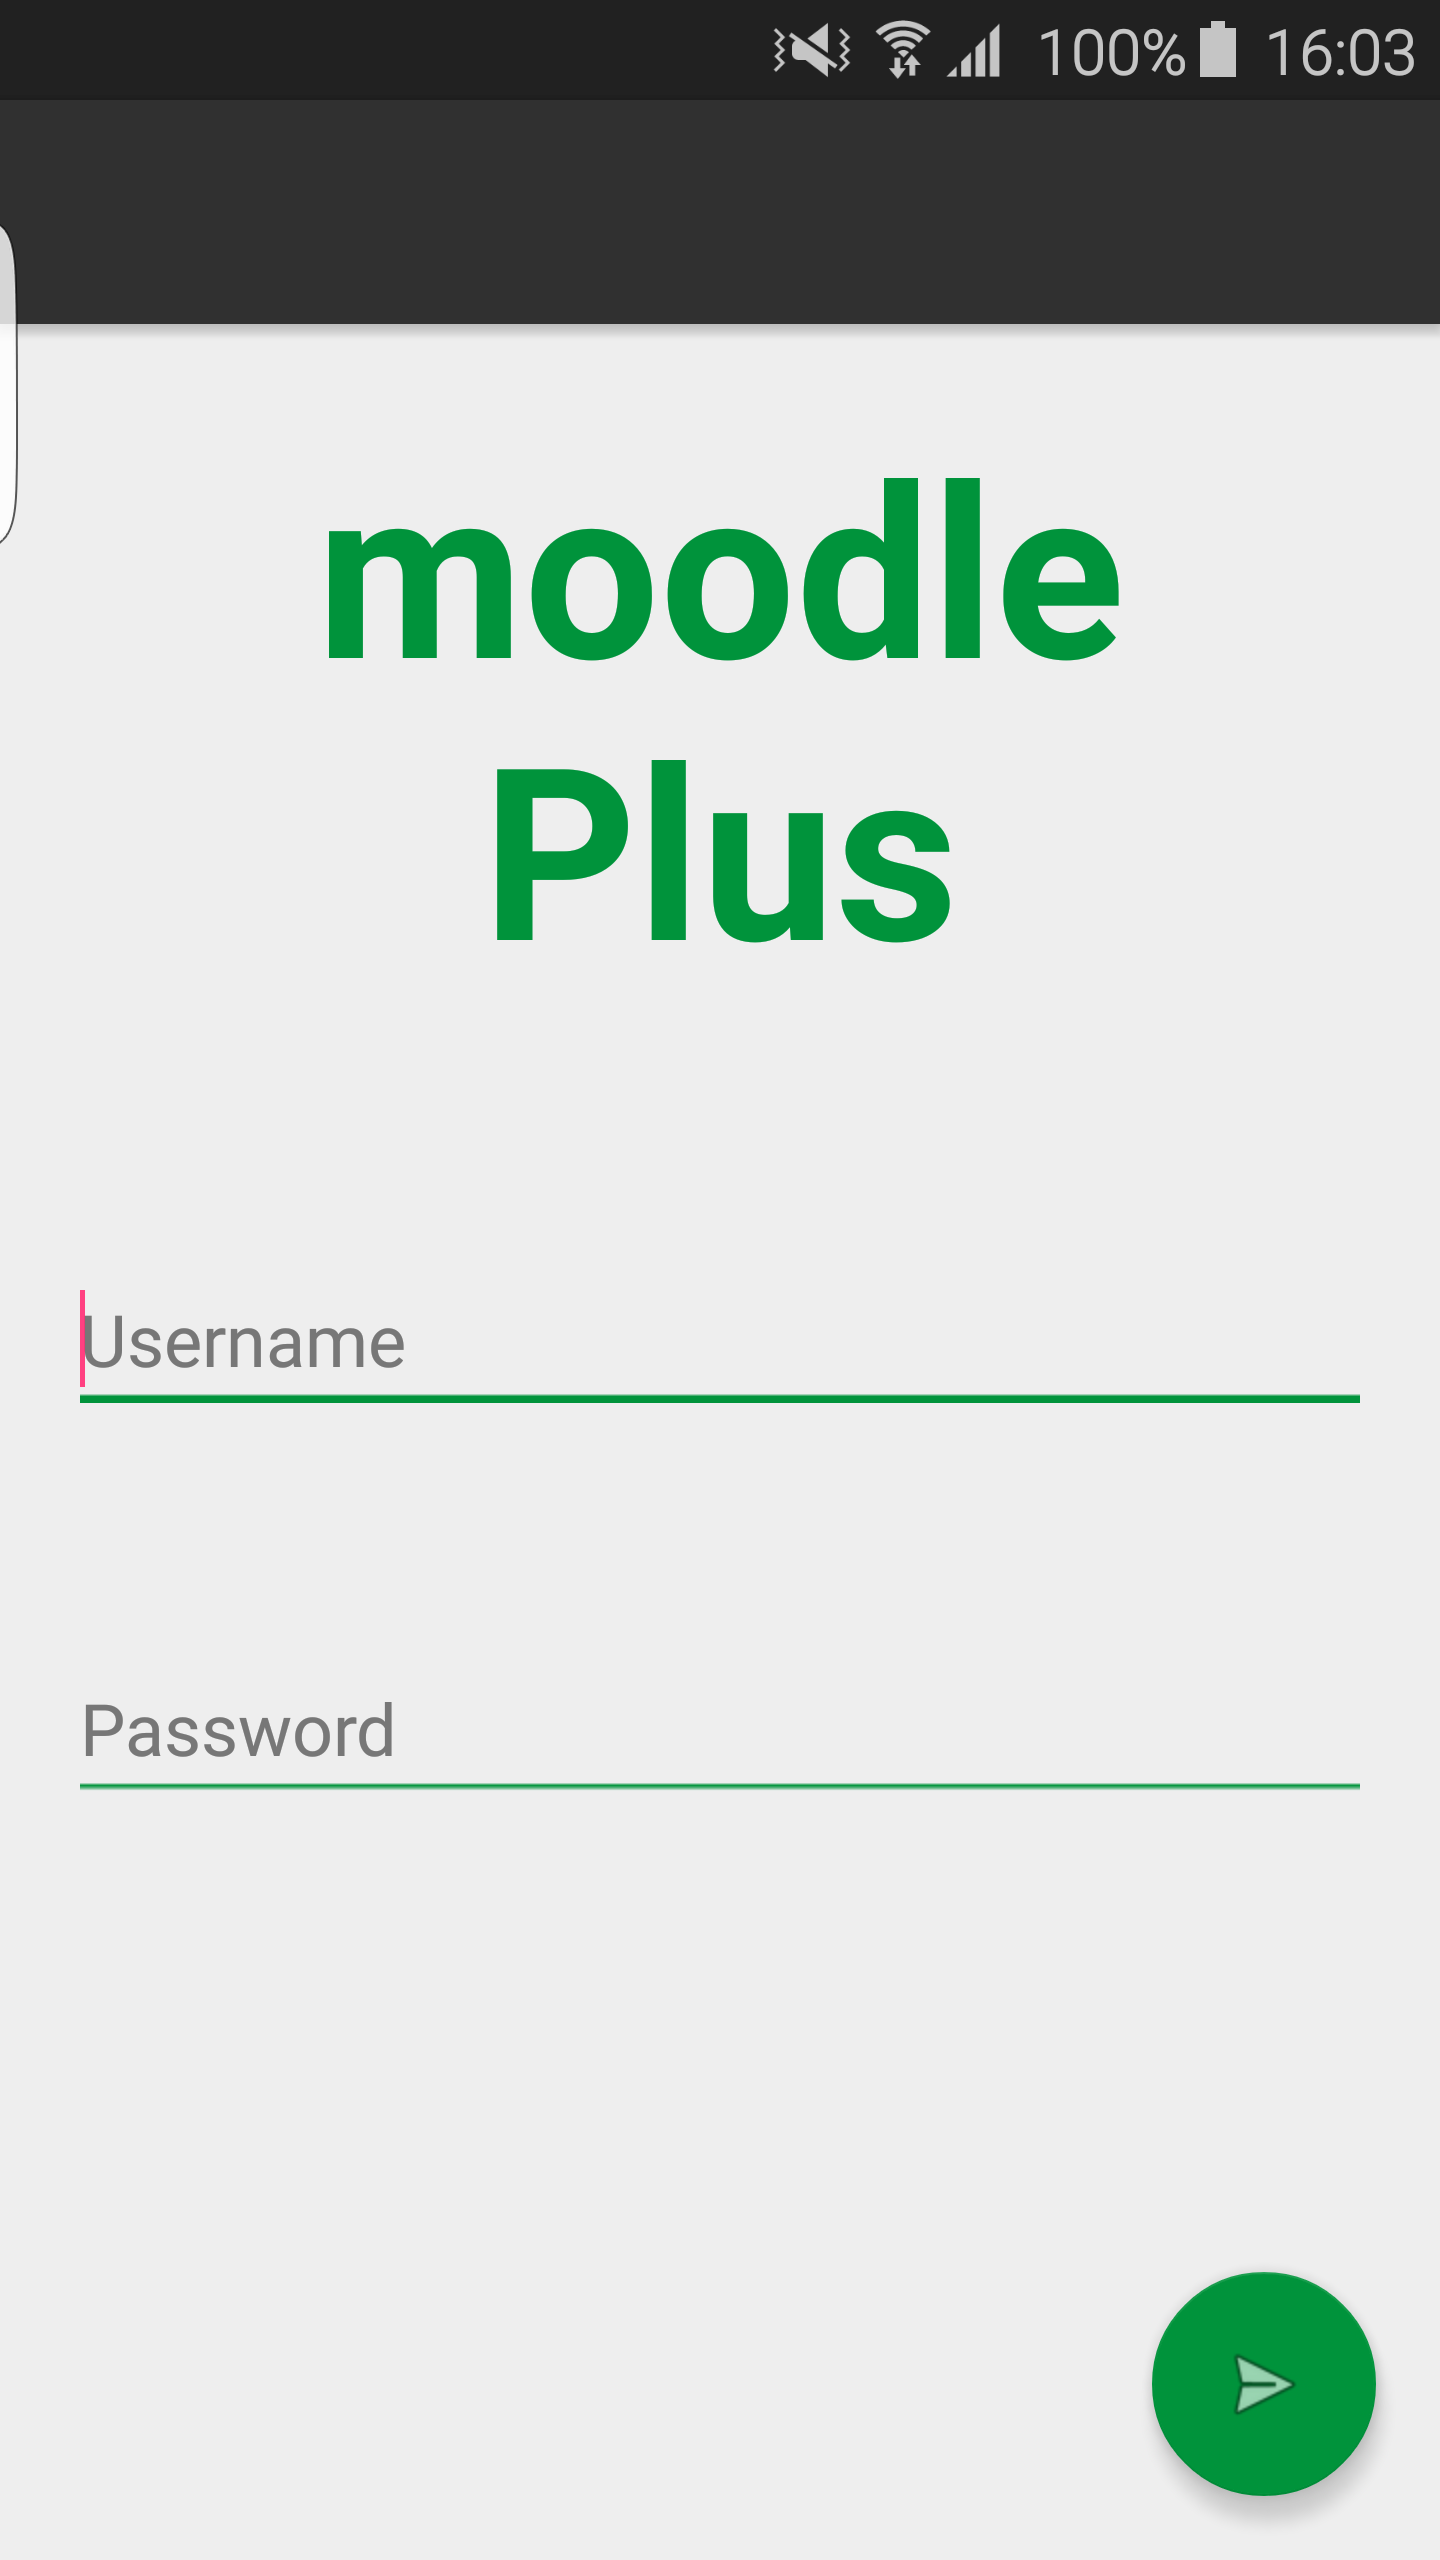
\includegraphics[width=\textwidth]{./LoginPage}
\captionsetup{justification=raggedright, singlelinecheck=false}
\captionof{figure}{Login Page}
\end{minipage}%
% \begin{minipage}[t]{.1\textwidth}
&
% \end{minipage}
\begin{minipage}[t]{.3\textwidth}
 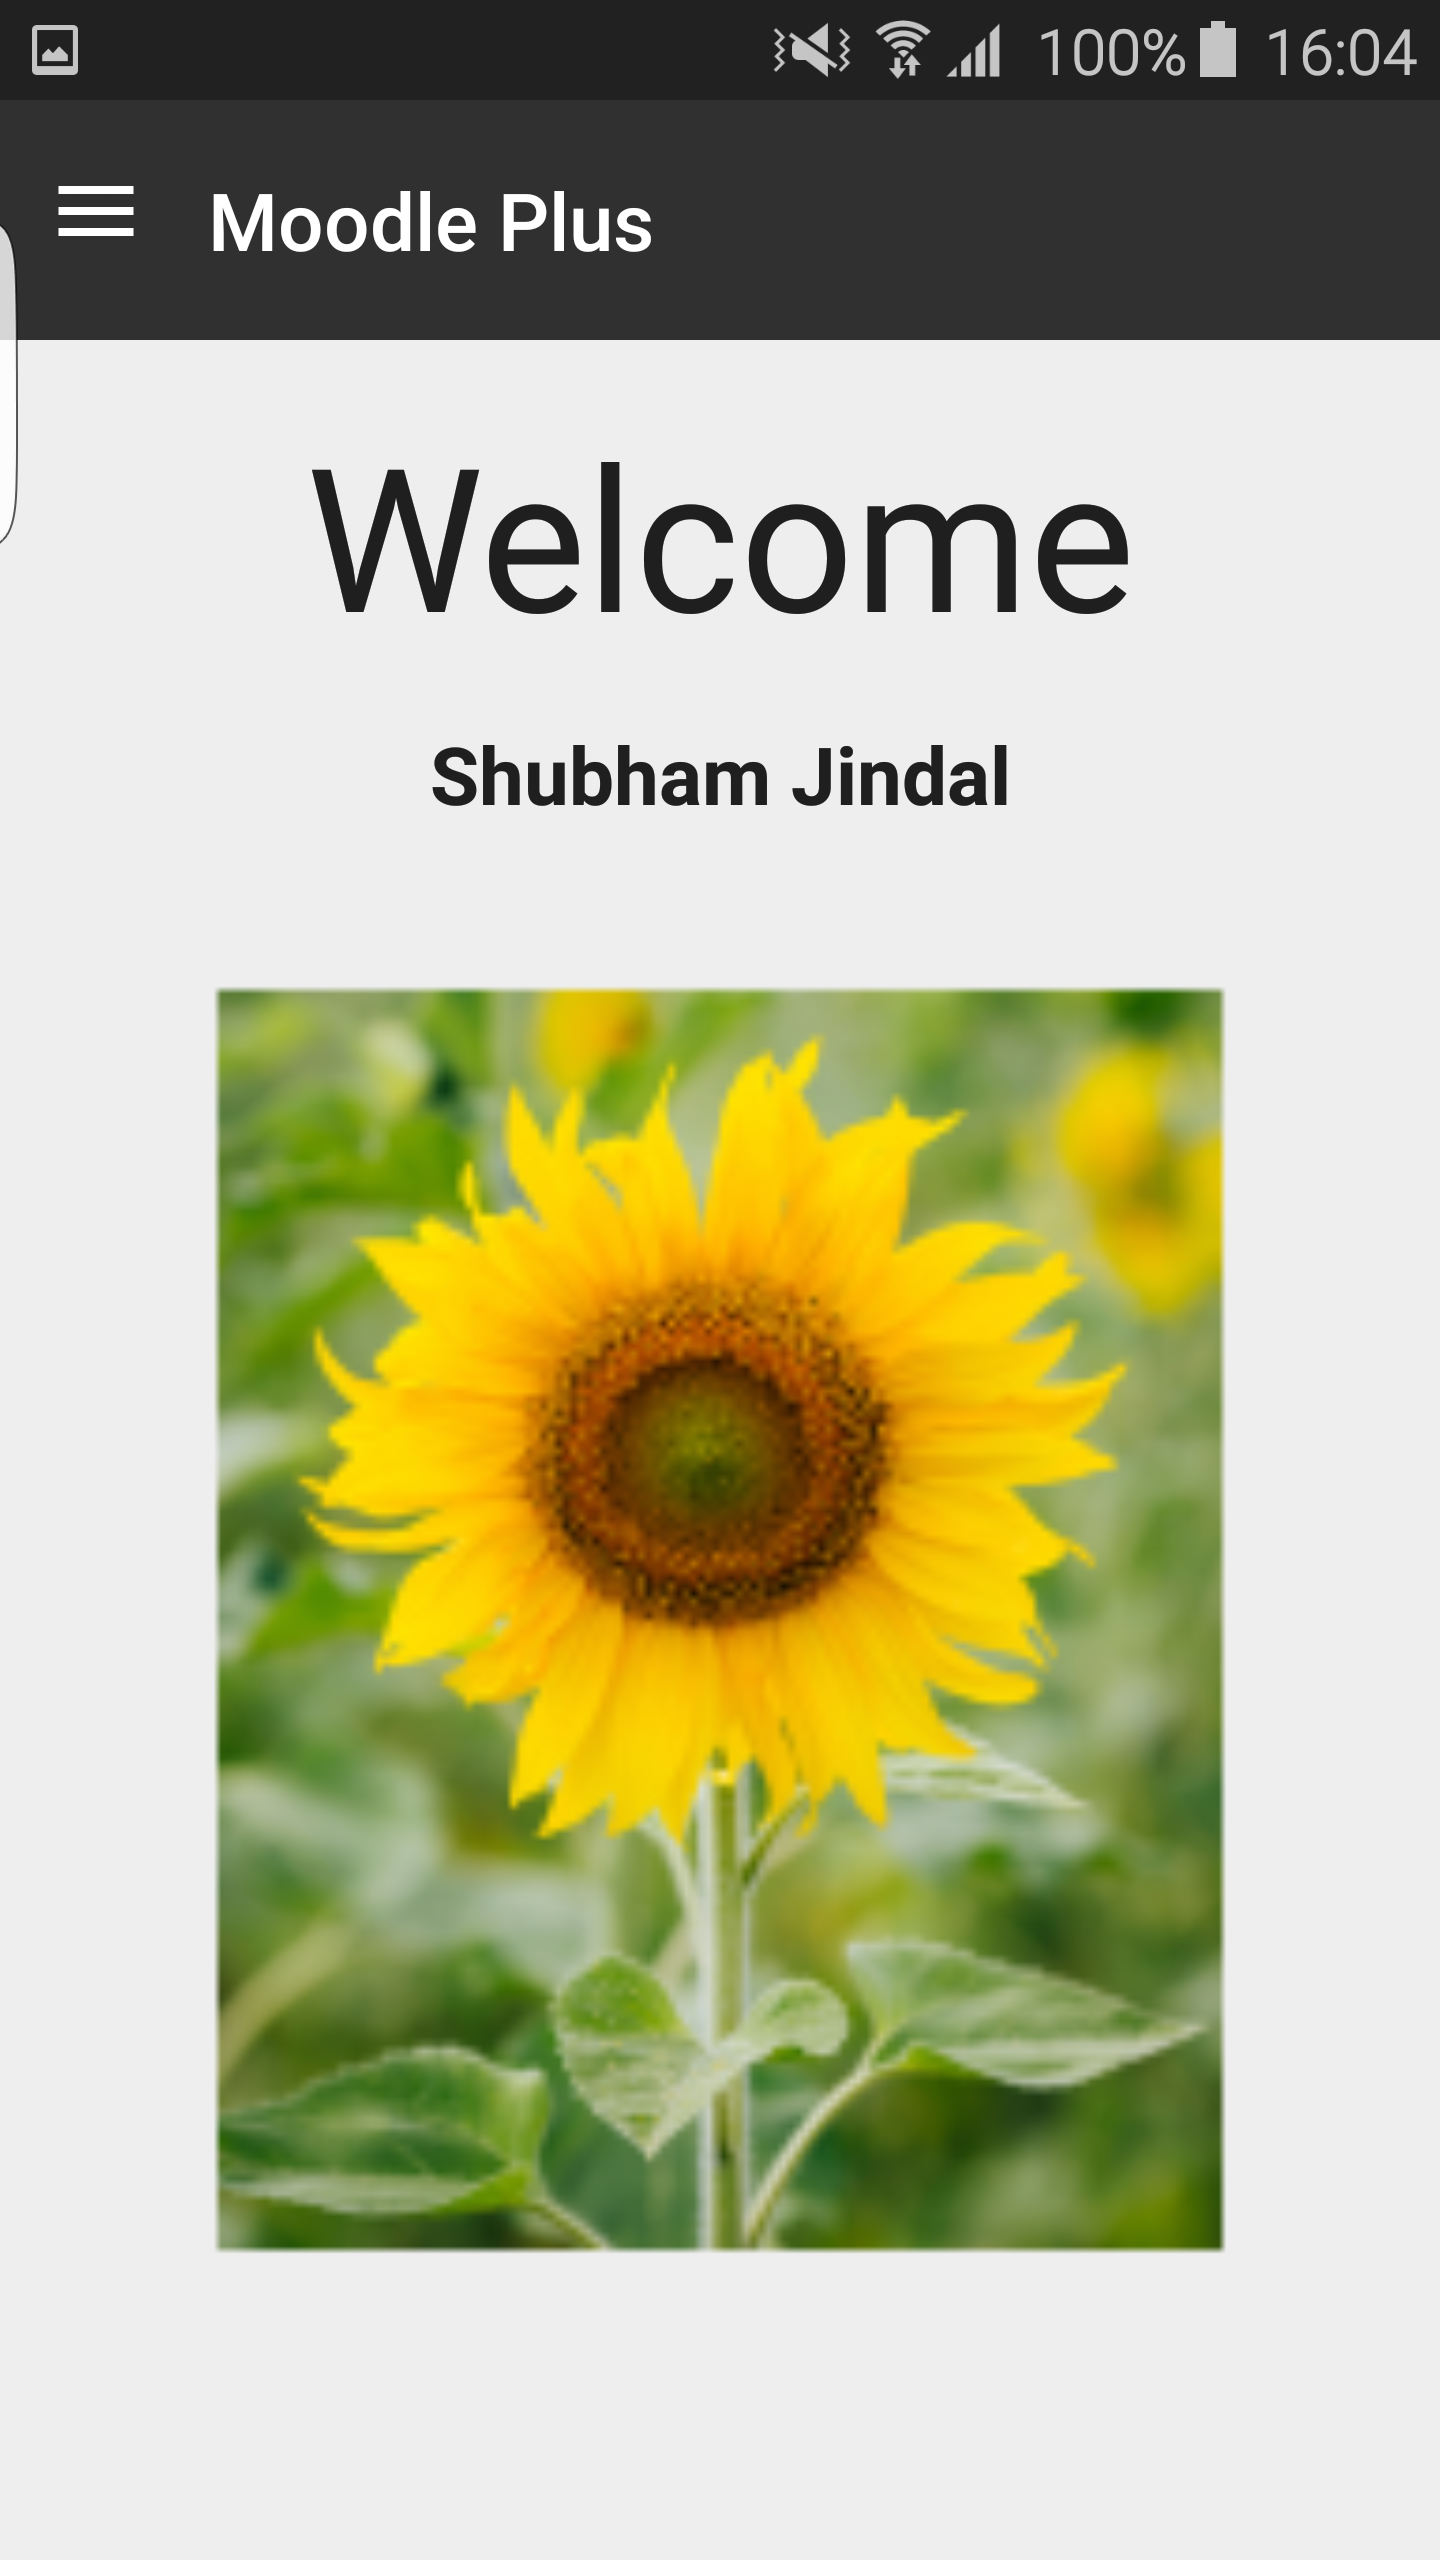
\includegraphics[width=\textwidth]{./HomePage}
 \captionsetup{justification=raggedright, singlelinecheck=false}
\captionof{figure}{Home Page}
\end{minipage}
% \begin{minipage}[t]{.1\textwidth}
& 
% \end{minipage}
\begin{minipage}[t]{.3\textwidth}
 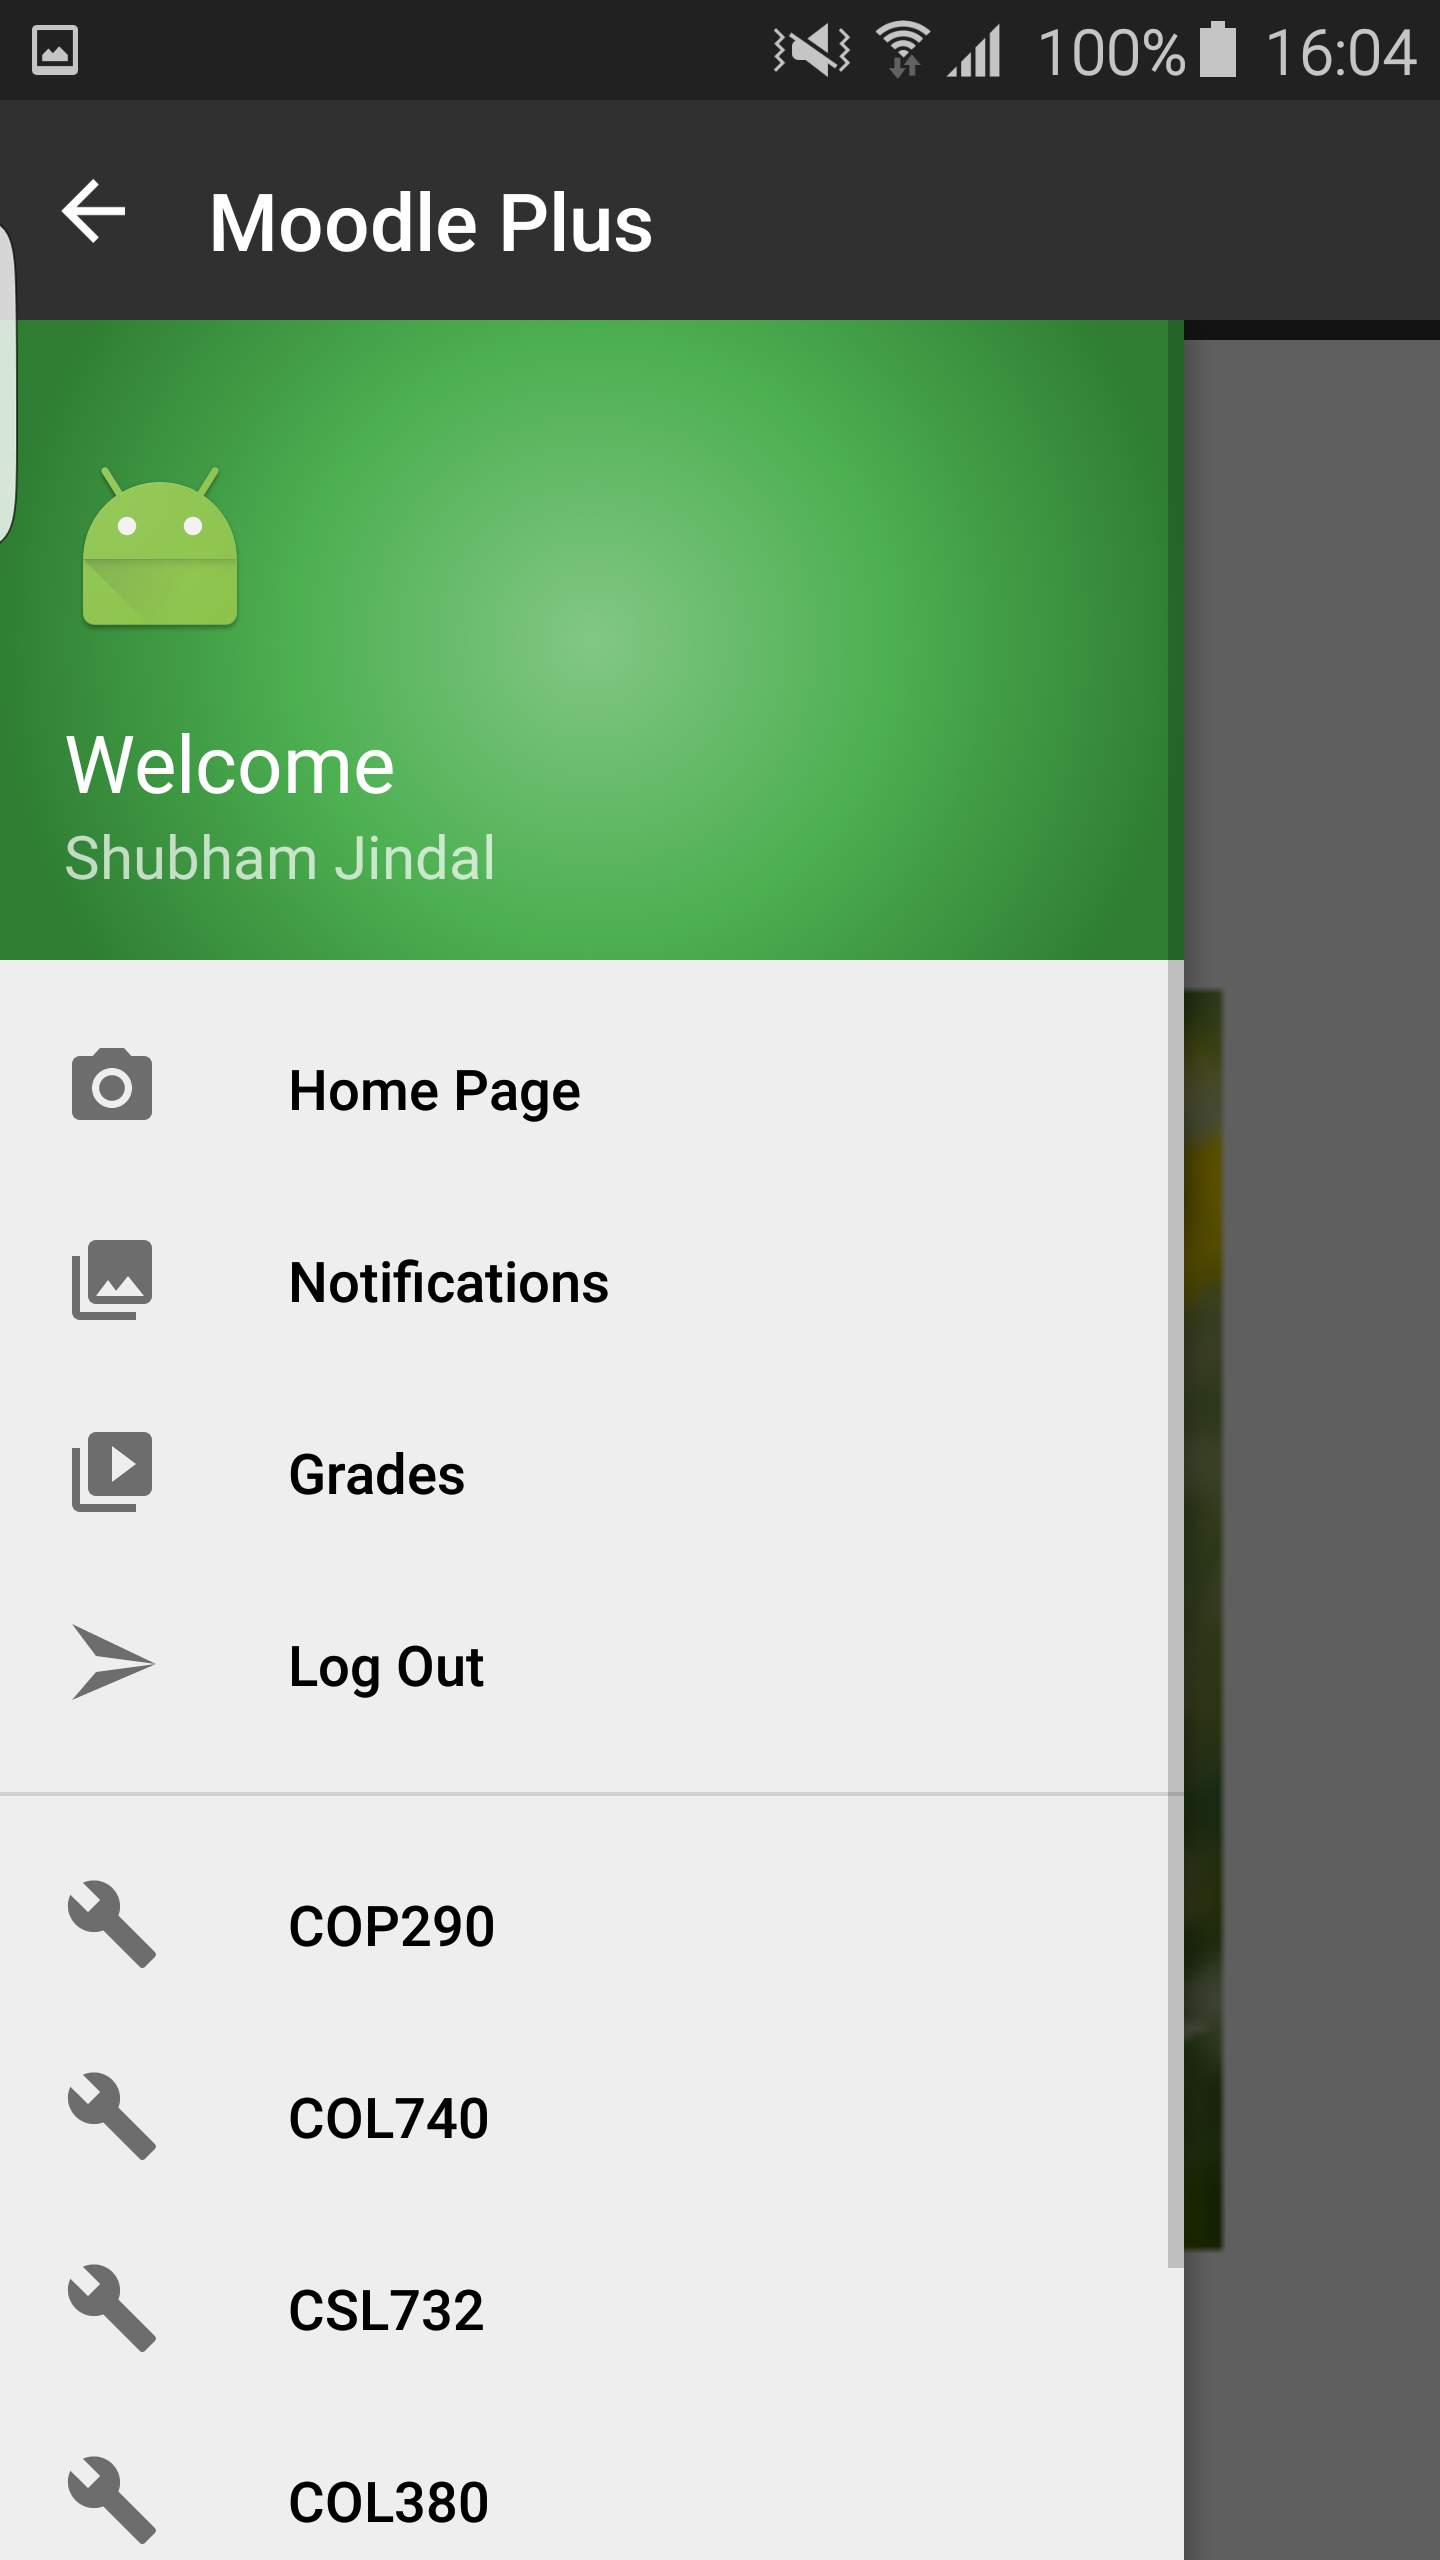
\includegraphics[width=\textwidth]{./NavDrawer}
 \captionsetup{justification=raggedright, singlelinecheck=false}
\captionof{figure}{Navigation Drawer}
\end{minipage}
  \\
\end{tabular}
\end{center}

\begin{itemize}
\item The user application contains the following screens for the functionality mentioned alongside:
    \begin{itemize}
        \item
        \begin{itemize}
        \item A \textbf{Login Screen} is encountered as the user opens the application prompting for the login credentials. The user proceeds by clicking the floating action button present on the screen
        \item On a successful login, the \textbf{Home Page Screen} appears. This home page screen contains a hidden \textbf{Navigation Drawer} which is accessible from the button on the top left. Apart from the navigation drawer, the Home Page also contains the Profile information of the user who has logged in
        \item The \textbf{Navigation Drawer} which shows up on clicking the button on the top left of the screen contains the pages to which the logged in user can navigate. It contains the links to the \textbf{Notification and Grades} page, the \textbf{list of courses} in which the user is registered and the \textbf{Link to Logout} off Moodle.
        \end{itemize}
    \end{itemize}    
\end{itemize}

\begin{center}
\begin{tabular}{c c c}
     
\begin{minipage}[t]{.3\textwidth}
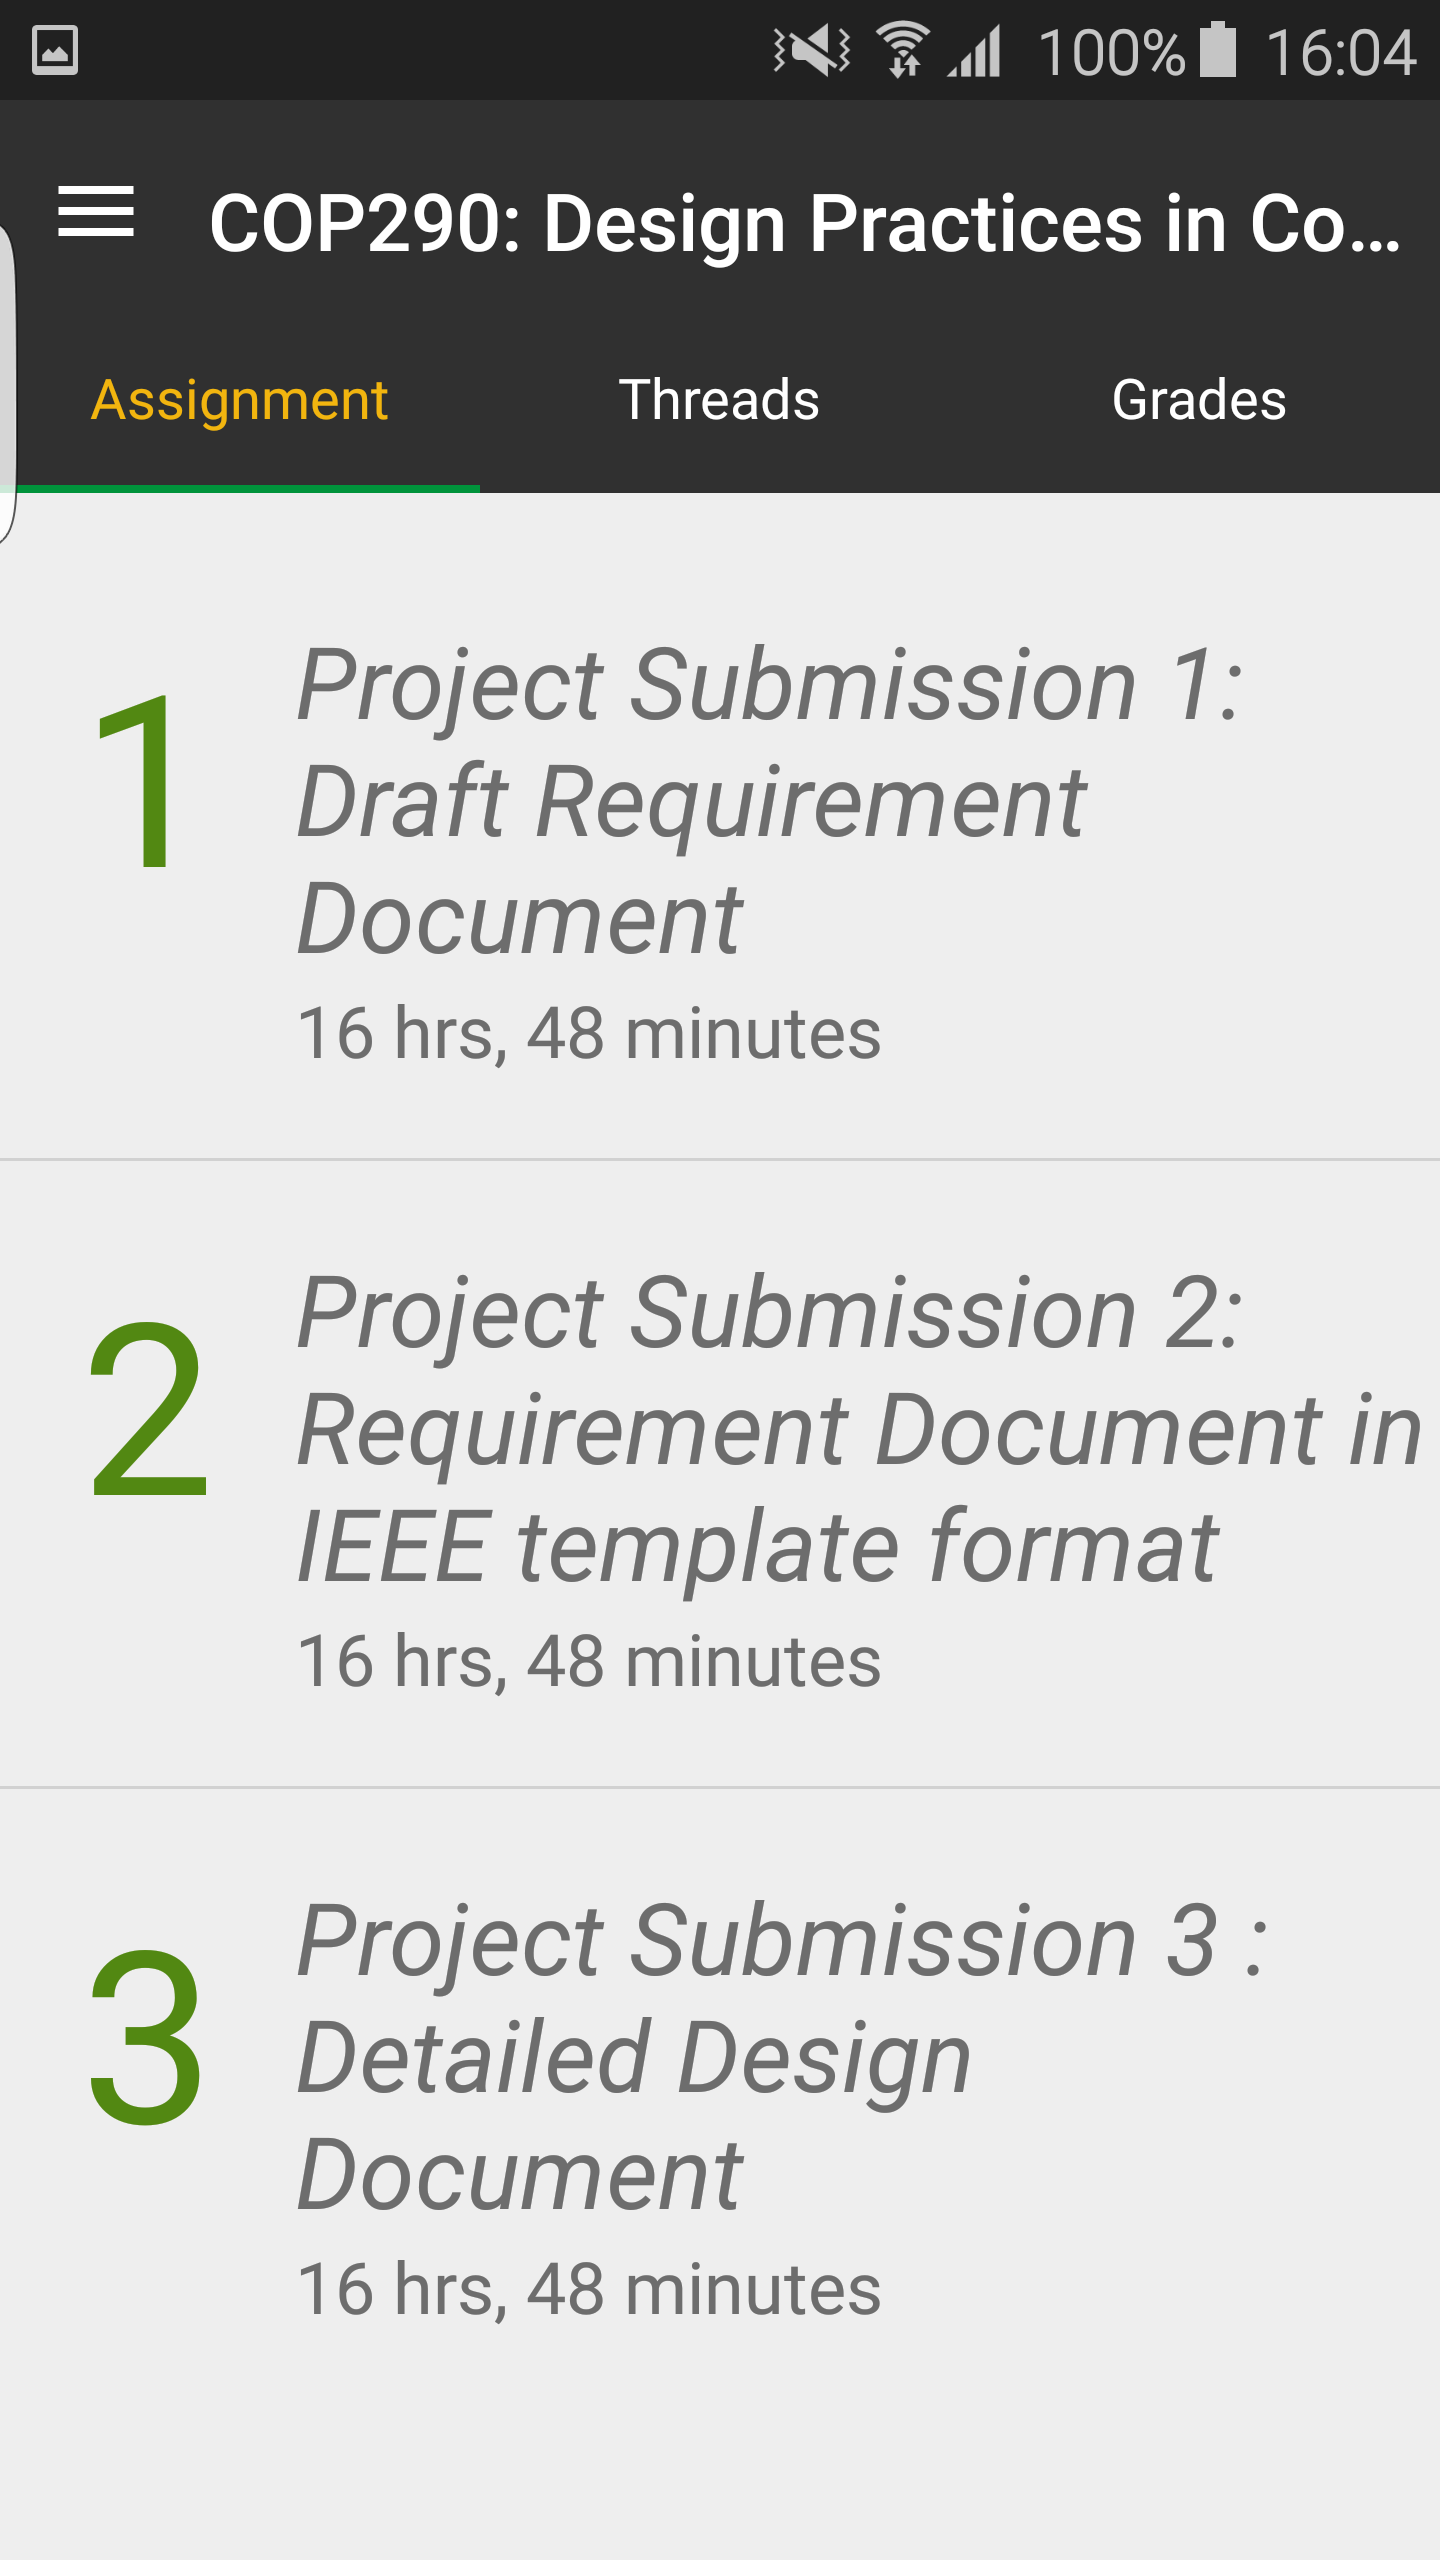
\includegraphics[width=\textwidth]{./Assignments}
\captionsetup{justification=raggedright, singlelinecheck=false}
\captionof{figure}{Assignment Page}
\end{minipage}%
% \begin{minipage}[t]{.1\textwidth}
&
% \end{minipage}
\begin{minipage}[t]{.3\textwidth}
 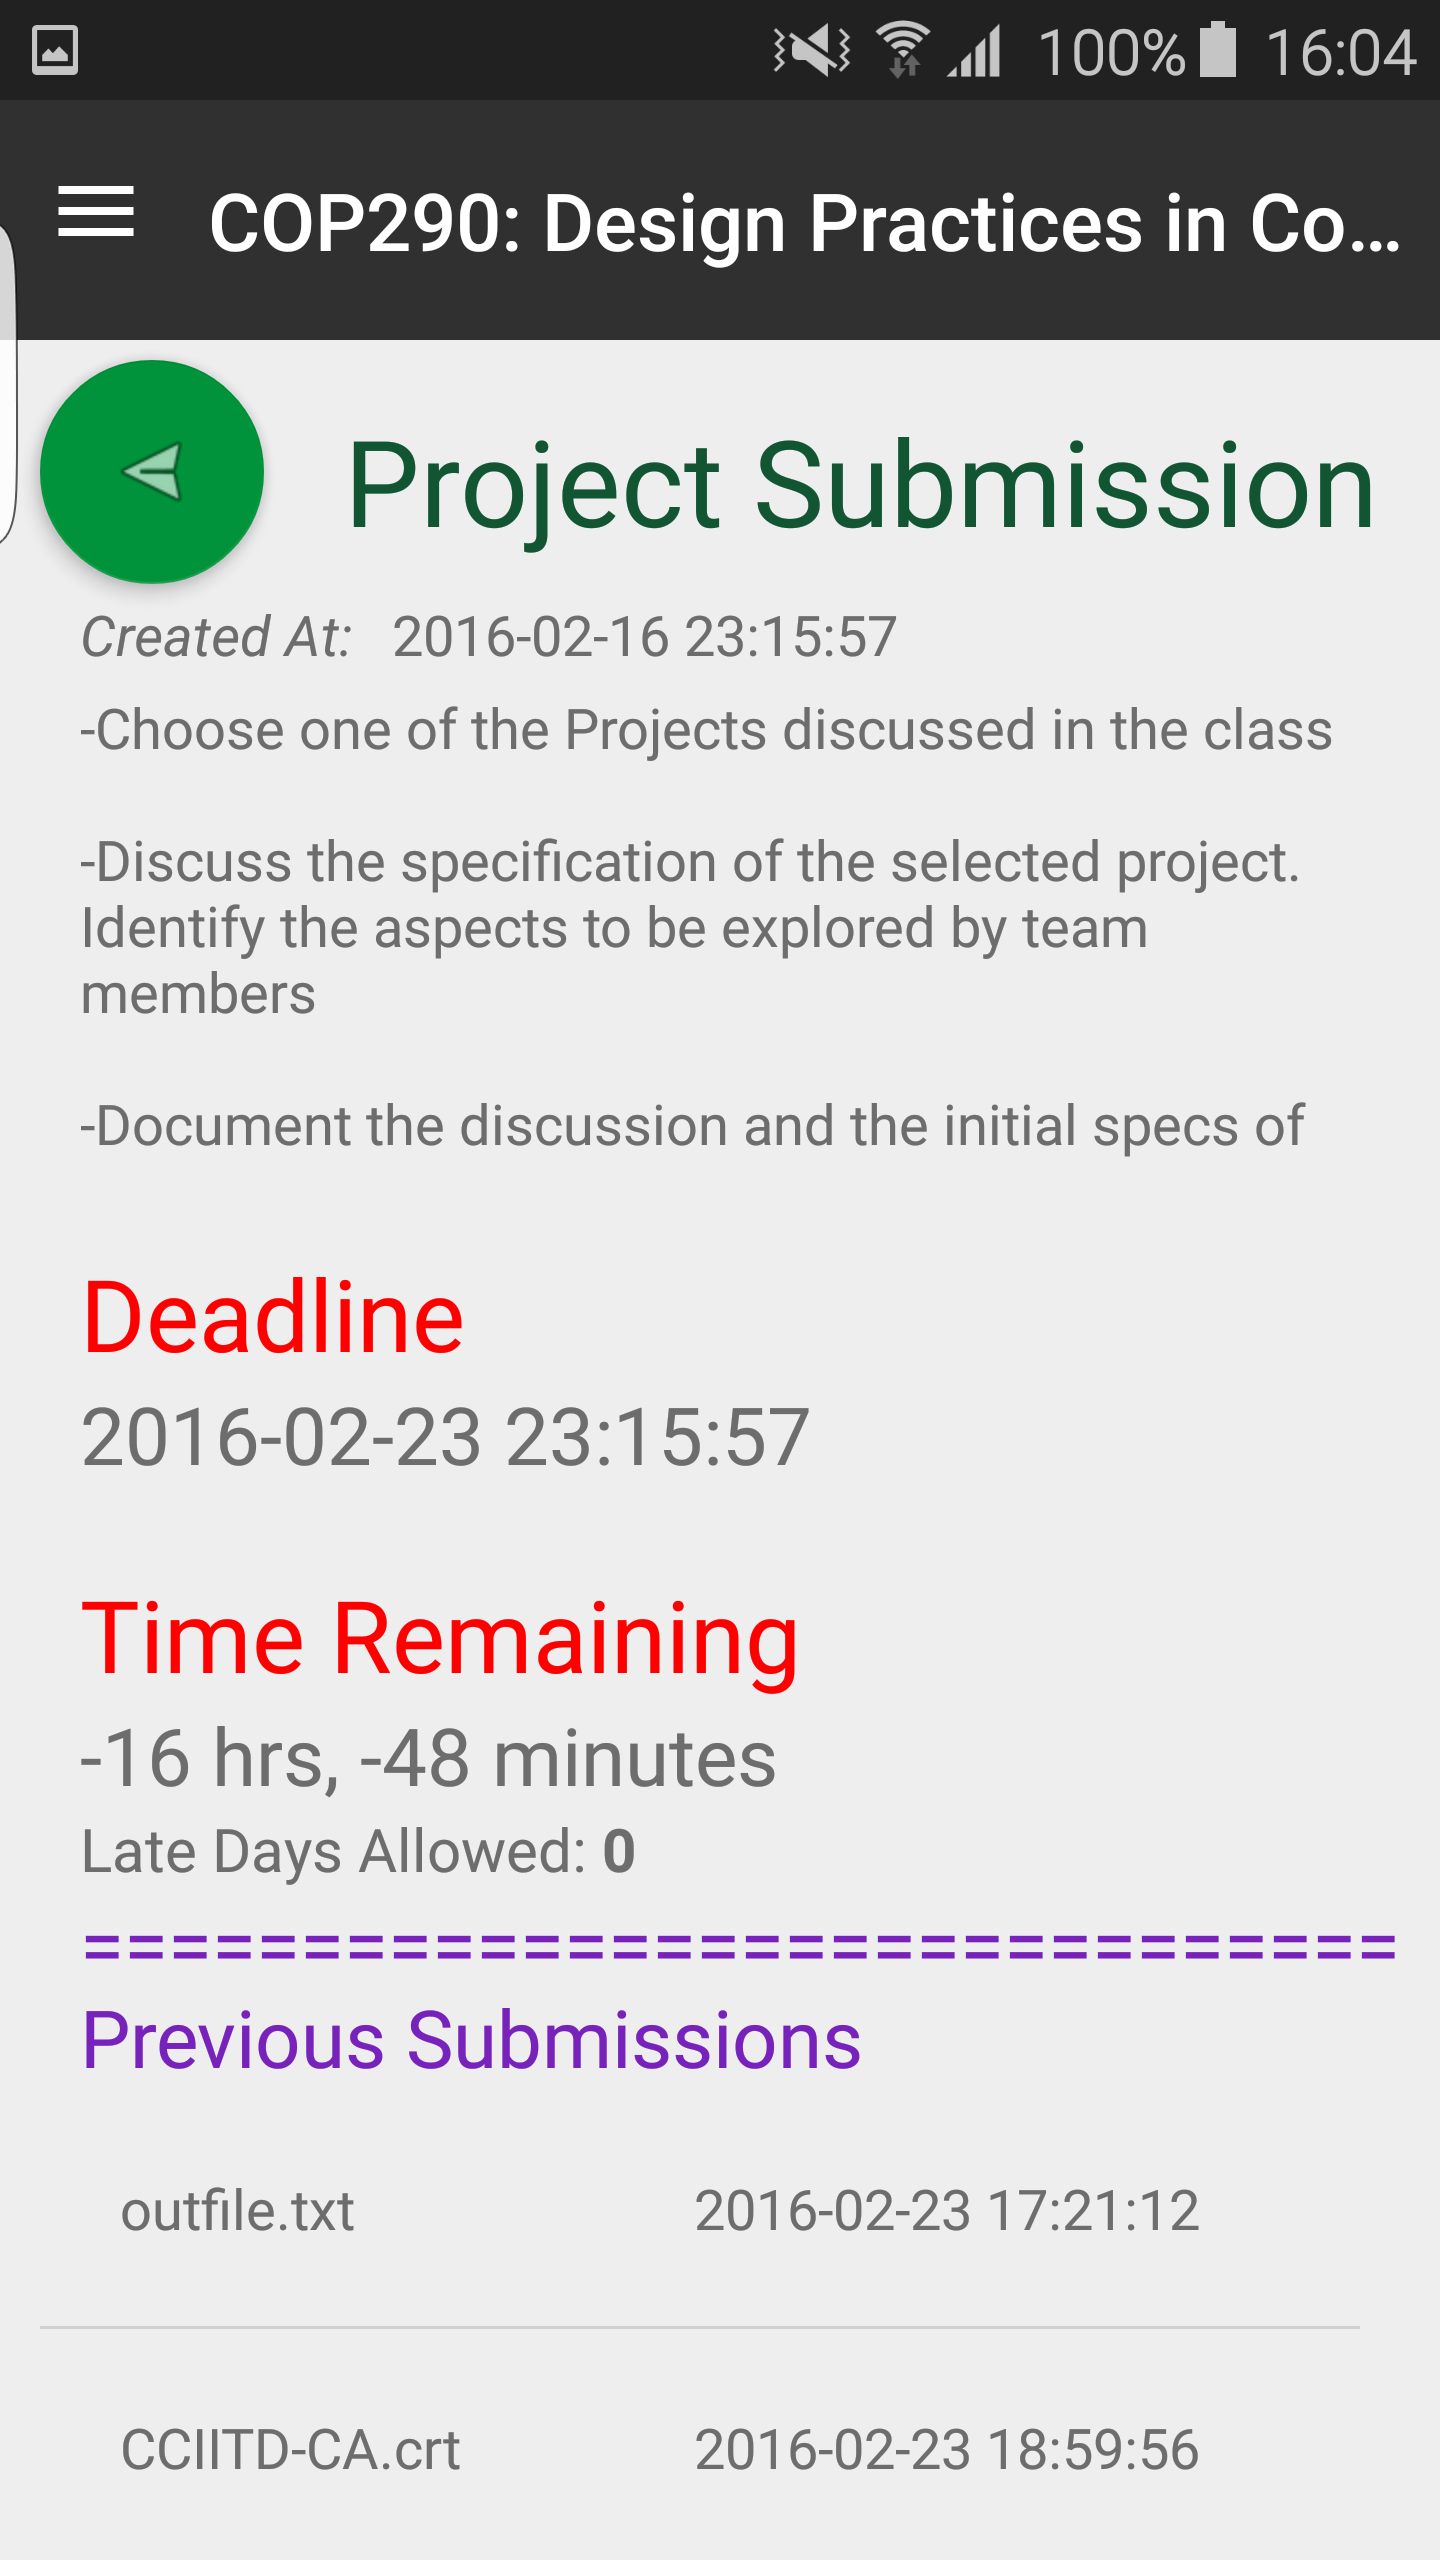
\includegraphics[width=\textwidth]{./ParticularAssignment}
 \captionsetup{justification=raggedright, singlelinecheck=false}
\captionof{figure}{Assignment Detail}
\end{minipage}
% \begin{minipage}[t]{.1\textwidth}
& 
% \end{minipage}
\begin{minipage}[t]{.3\textwidth}
 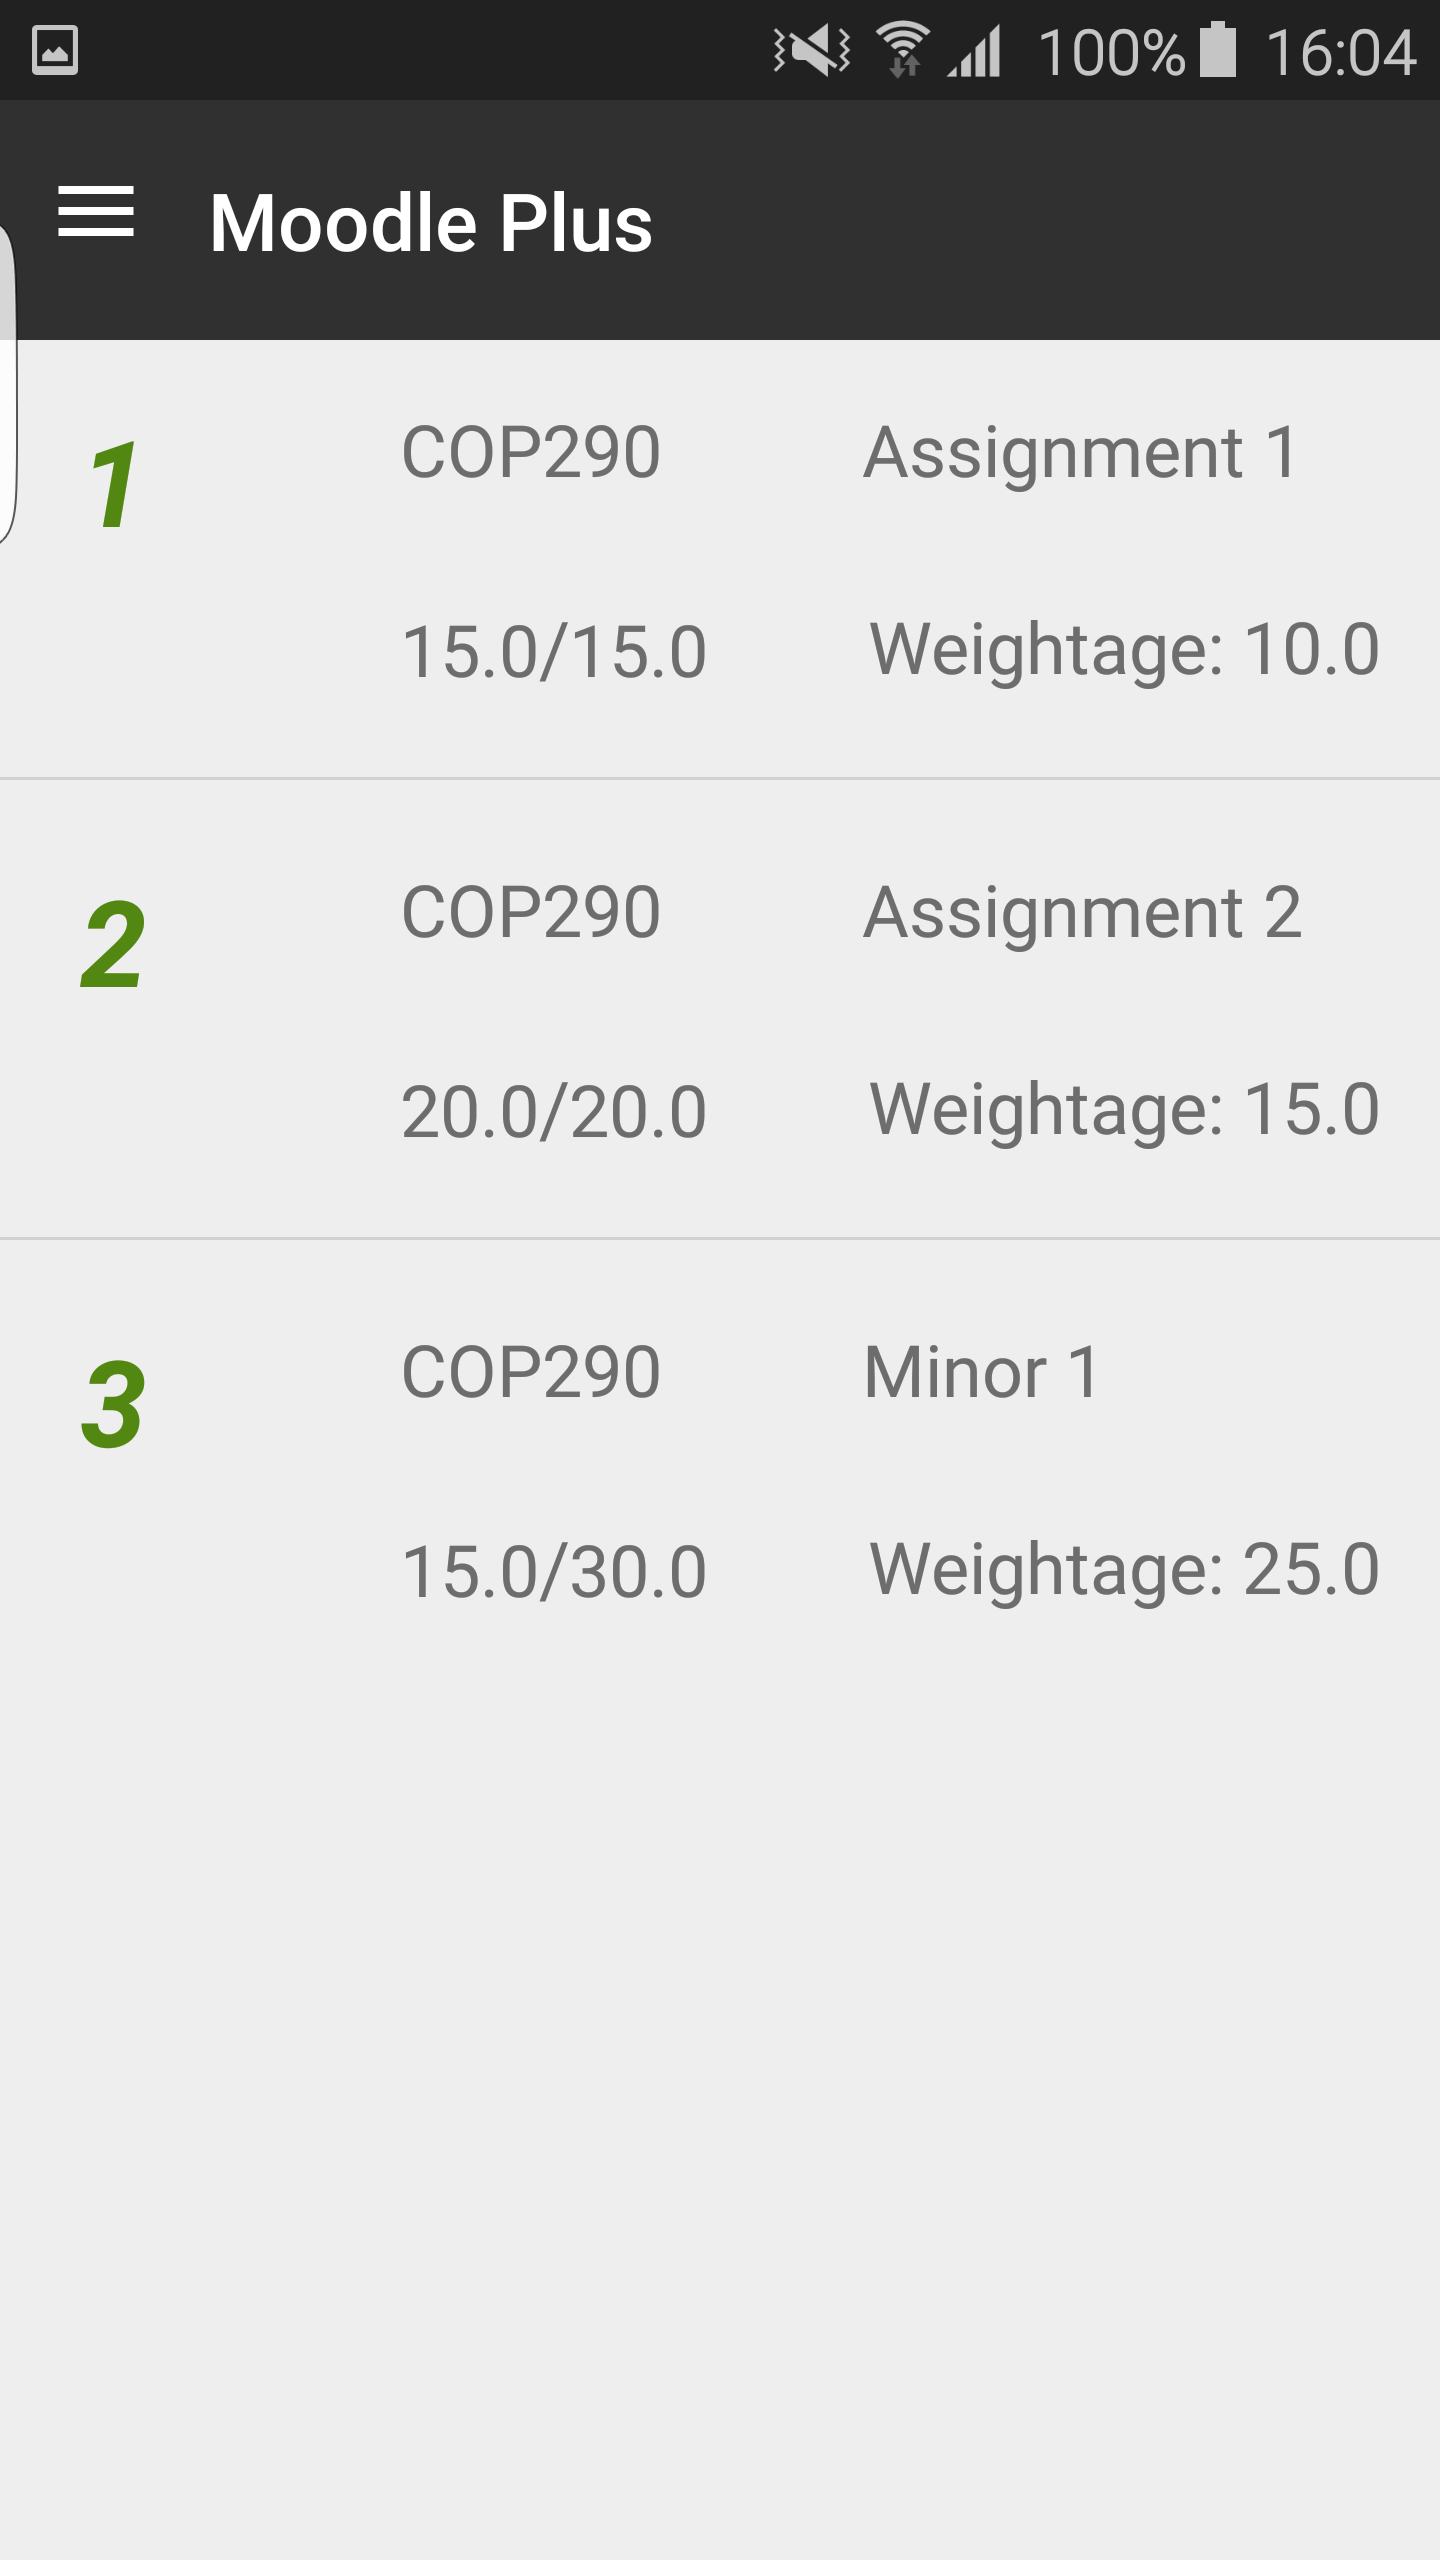
\includegraphics[width=\textwidth]{./Grades}
 \captionsetup{justification=raggedright, singlelinecheck=false}
\captionof{figure}{Grades Page}
\end{minipage}
  \\
\end{tabular}
\end{center}

\begin{itemize}
    \item
    \begin{itemize}
        \item
        \begin{itemize}
        \item The \textbf{Course Home Page} which shows up on clicking the Course code on the navigation drawer is the Home page of a given course. It contains three fragments \textbf{Assignments, Threads and Grades} which can be accessed by swiping towards left or right on the course Home Page.
        \item The \textbf{Assignments Fragment} of the Course home page contains the list of assignments along with their titles and times remaining for deadlines. The details of a \textbf{Particular Assignment} can be accessed by clicking on the title of the relevant assignment whose details you want to access.
        \item The \textbf{Threads Fragment} of the Course home page contains the list of course threads along with their titles and descriptions. The details of a \textbf{Particular Thread} can be accessed by clicking on the title of the relevant thread whose details you want to access.
        \item The \textbf{Grades Fragment} of the Course home page contains the list of course grades of the student.
        \end{itemize}
        \item
        \begin{itemize}
        \item The \textbf{Notifications Page} which shows up on clicking the Notifications tab on the navigation drawer is the page which shows the list of notifications. 
        \end{itemize}
        \item
        \begin{itemize}
        \item The \textbf{All Grades Page} which shows up on clicking the Grades tab on the navigation drawer is the page which shows the list of grades of the user in all the courses he has registered for. 
        \end{itemize}
    \end{itemize}
\end{itemize}

\newpage

\begin{center}
\begin{tabular}{c c c}
     
\begin{minipage}[t]{.3\textwidth}
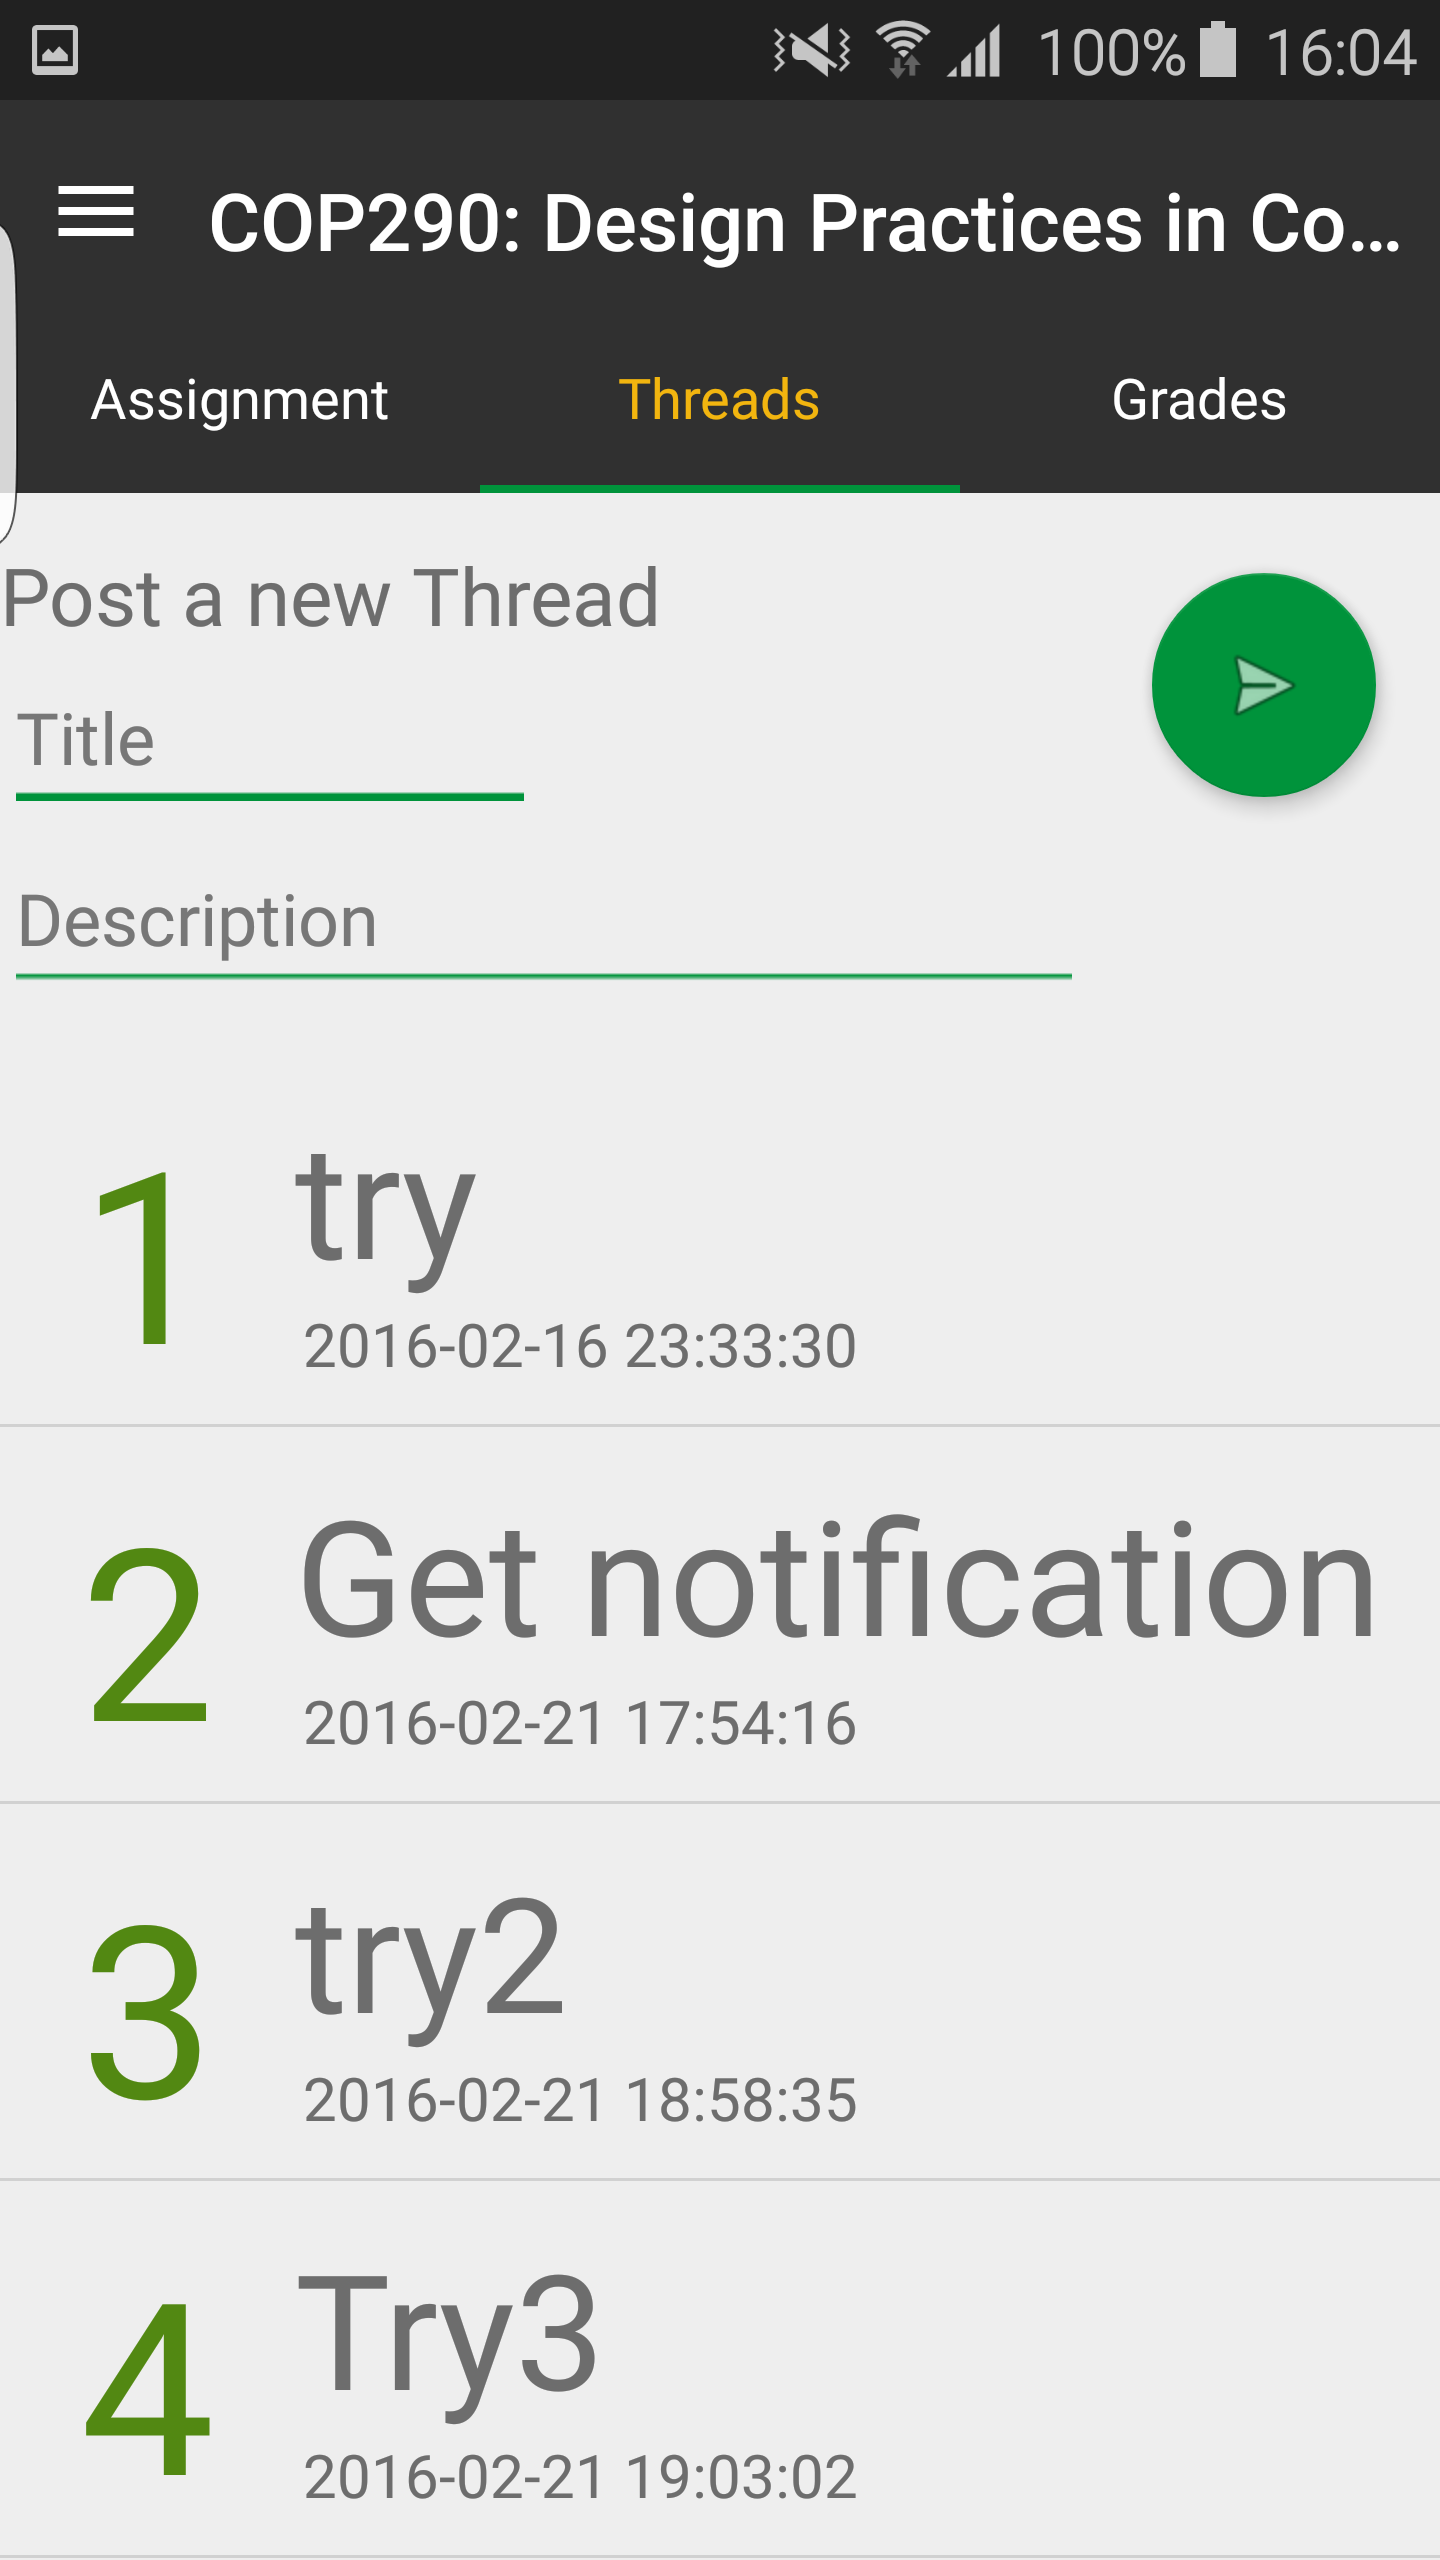
\includegraphics[width=\textwidth]{./Threads}
\captionsetup{justification=raggedright, singlelinecheck=false}
\captionof{figure}{Threads Page}
\end{minipage}%
% \begin{minipage}[t]{.1\textwidth}
&
% \end{minipage}
\begin{minipage}[t]{.3\textwidth}
 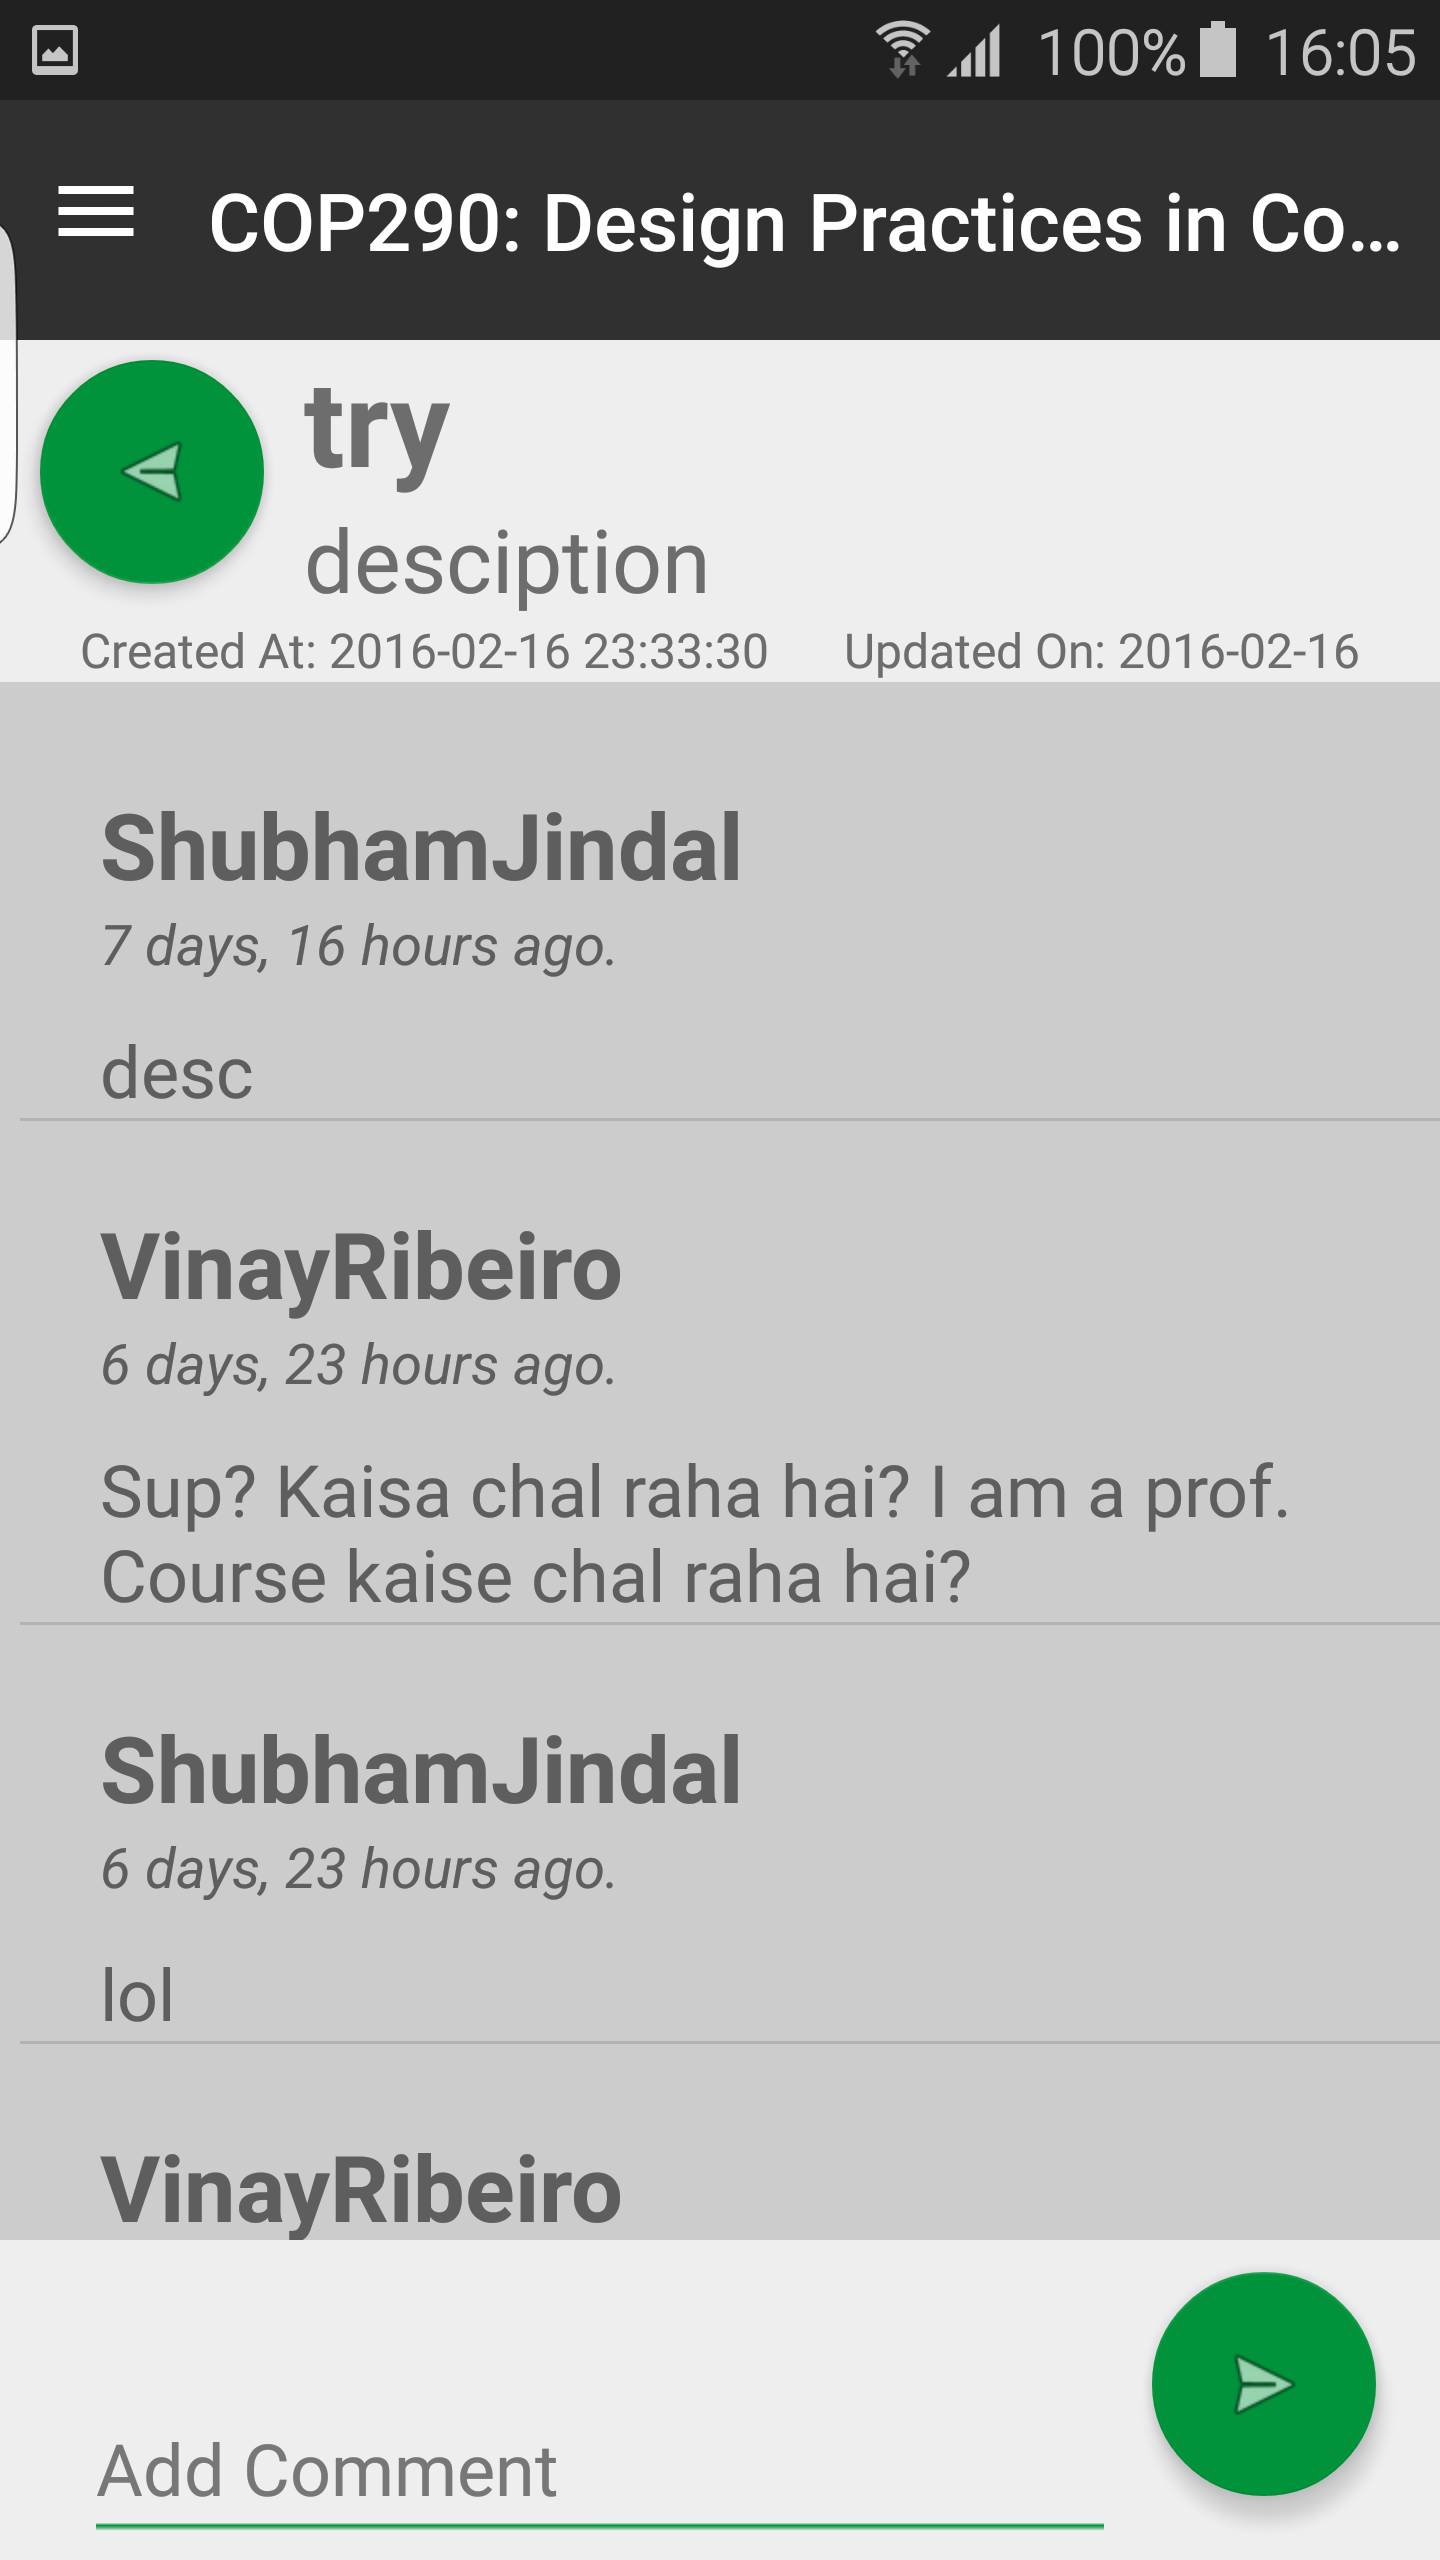
\includegraphics[width=\textwidth]{./ParticularThread}
 \captionsetup{justification=raggedright, singlelinecheck=false}
\captionof{figure}{Thread Detail}
\end{minipage}
% \begin{minipage}[t]{.1\textwidth}
& 
% \end{minipage}
\begin{minipage}[t]{.3\textwidth}
 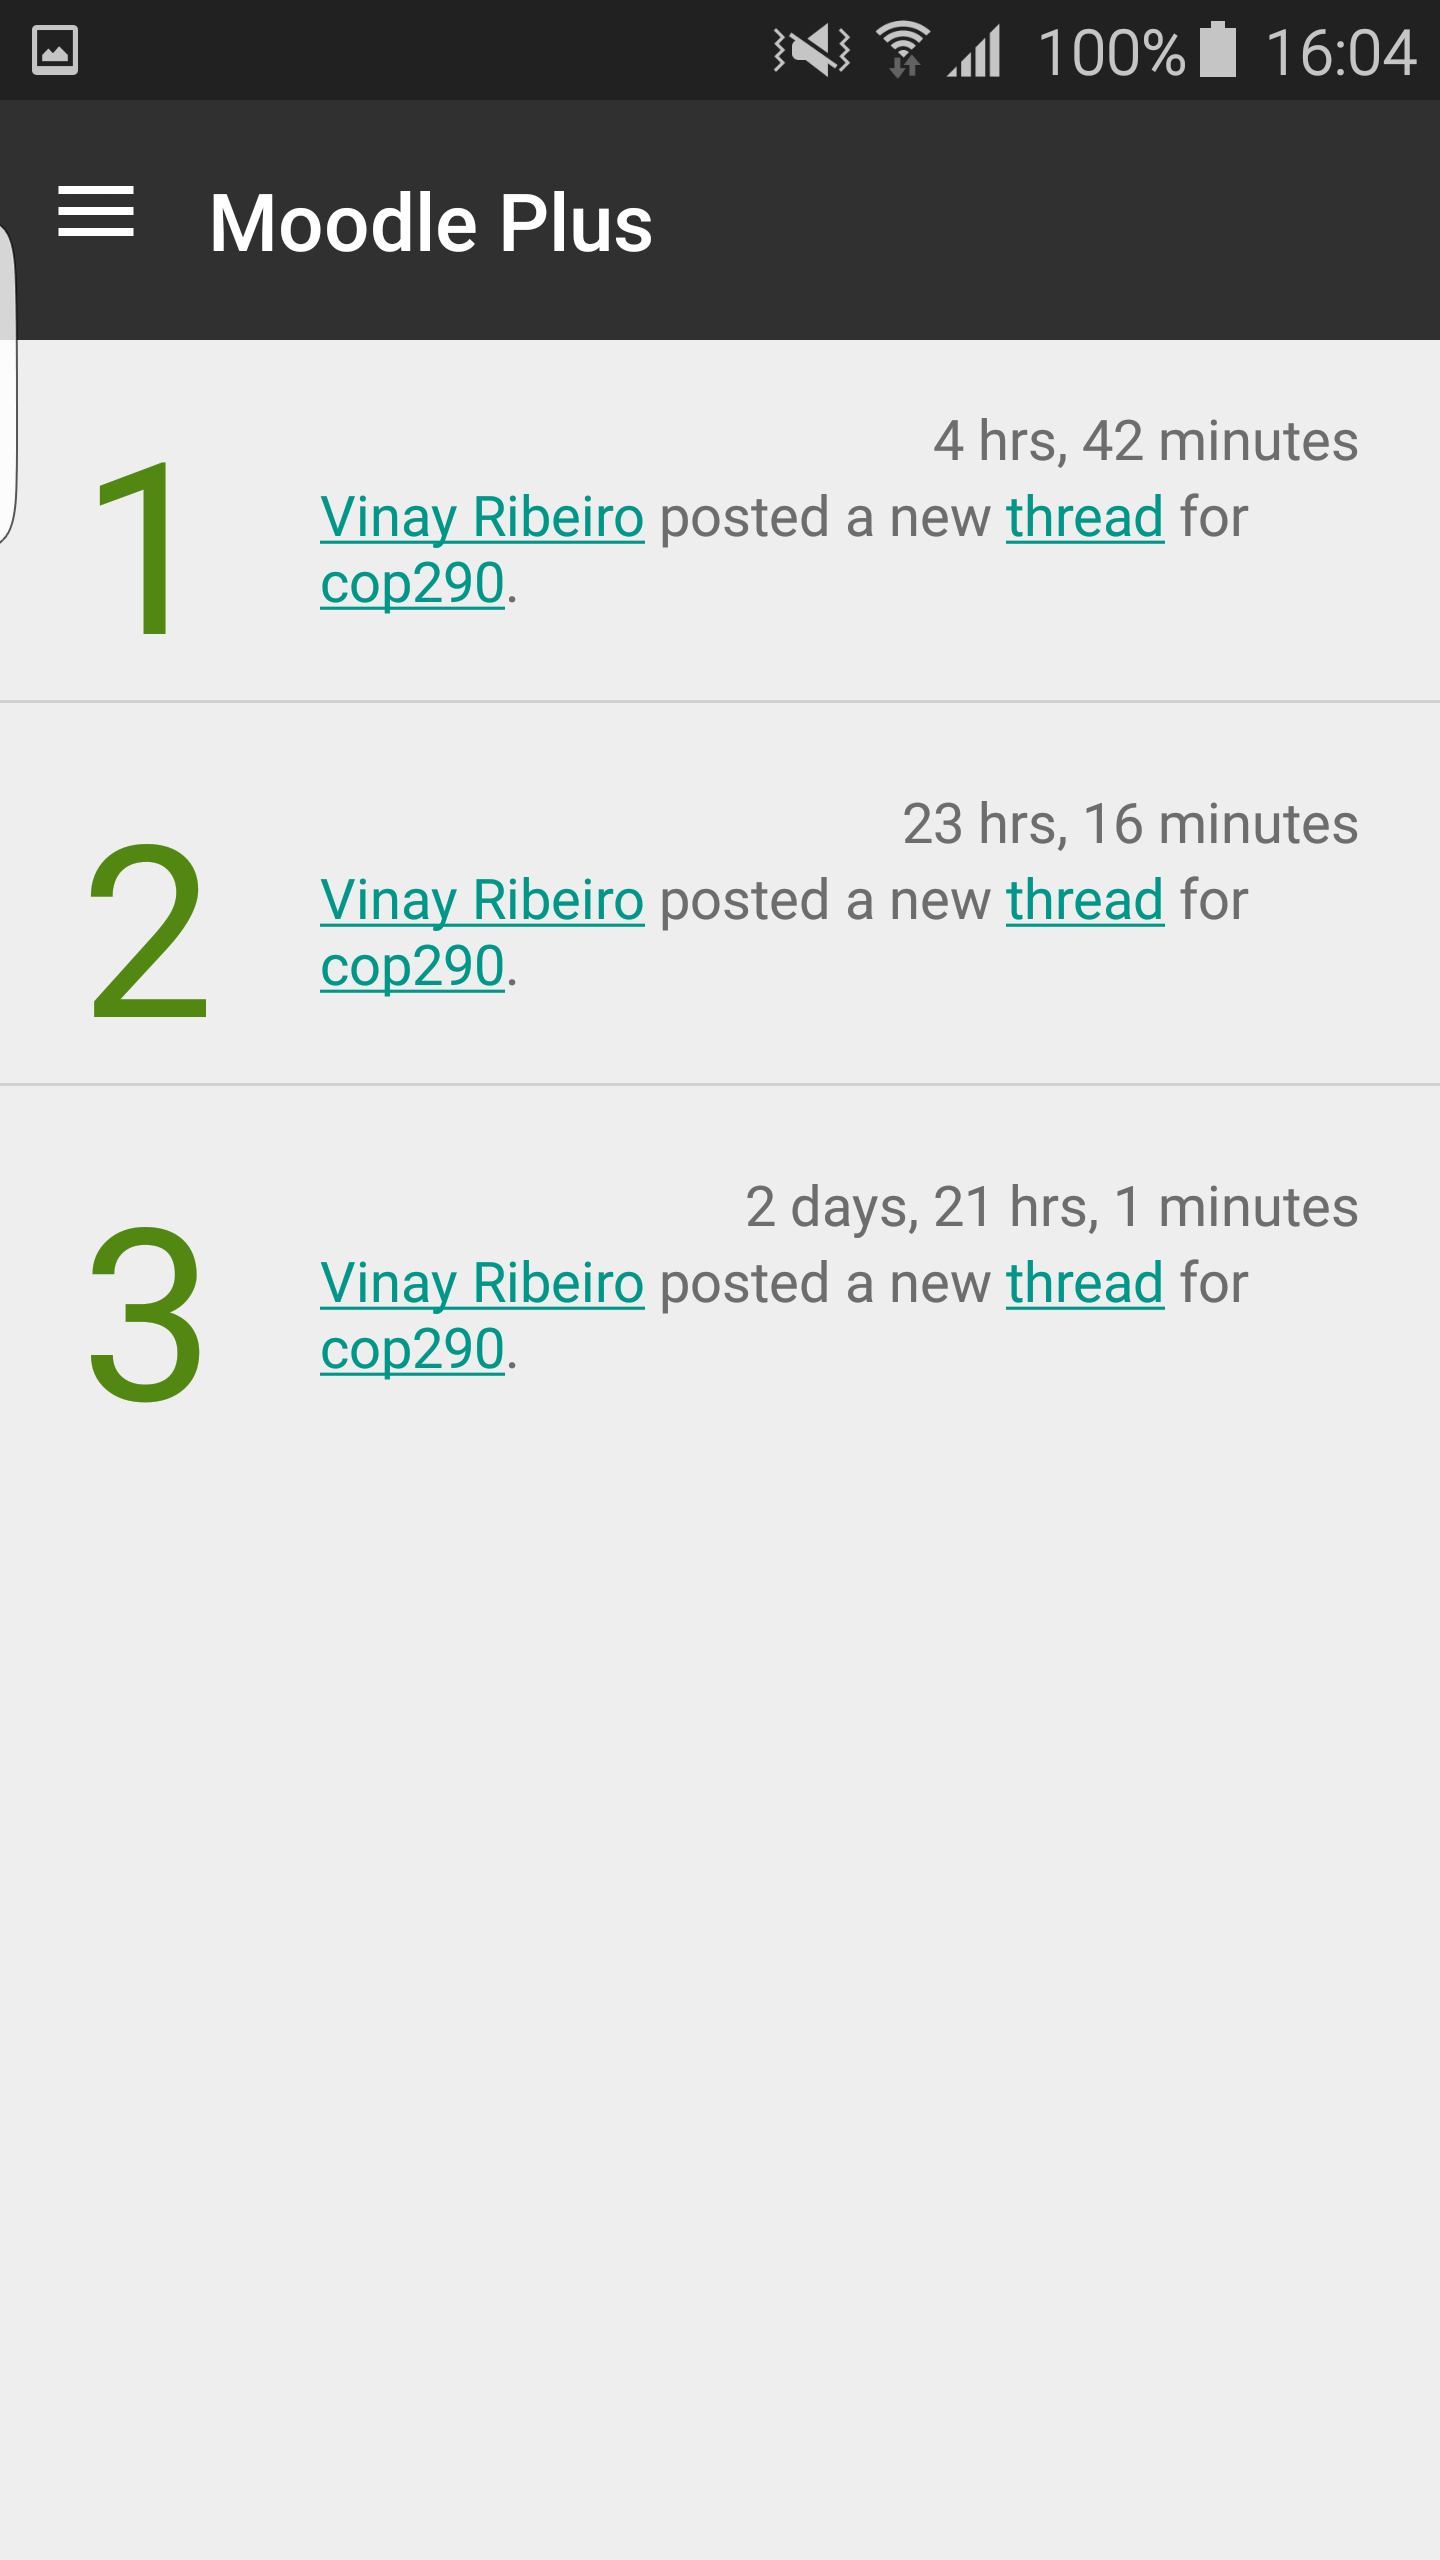
\includegraphics[width=\textwidth]{./Notifications}
 \captionsetup{justification=raggedright, singlelinecheck=false}
\captionof{figure}{Notifications Page}
\end{minipage}
  \\
\end{tabular}
\end{center}

\begin{itemize}
\item \begin{itemize}

    \item The functionality of refresh has been given to the user through the \textbf{Swipe Refresh}. Once the user refreshes, the app will go to the home page and refresh the data from the server.
    
    \end{itemize}
\item 
\begin{itemize}
    \item The appropriate data validations are imposed on creating new comments and threads, and error messages in form of an Alerts and Toasts are flashed if the data is found to be of an incorrect format.  
\end{itemize}
\end{itemize}

\section{Implementation Details~\cite{developer_android}~\cite{stack_overflow}}

\begin{itemize}
\item The application makes GET requests to the locally hosted server and gets a JSON response. Modularity has been ensured in interaction of application with the server and Parsing of the JSON objects to extract relevant information.
\item There is a single static class which is responsible for interaction of the server and the application. The class contains methods which take in the parameters (when required), make the GET requests to the endpoints mentioned in the problem statement and wait for the responses using callbacks. The String responses are registered as data items in the static class and are accessed by the JSON parsing objects. This eliminates the need of passing the required data using bundles to other activities in the application and makes changing the format of get requests easy.
\item
The basic problem which arises here is that the callbacks are asynchronous and one needs to move over to the subsequent fragments or pages once a response of the GET requests has been registered. To ensure this, each of the callback method sets a flag to true on response and further action is taken only when the flag is set to true. 
\item The parsing of JSON objects {~\cite{json_parse}} has also been done in a modular manner and every JSON response has a corresponding class associated with it. This takes in the string response and sets the data items of the class preserving the structure of the JSON data. Whenever a JSON object is to be parsed, the corresponding class' object is instantiated and parsing is done.
\item The user interface of the application has been created using a Navigation Drawer activity and Swiping activity using fragments. There are only twon activities in the application - Login and the Home Page. The notifications, grades, threads, assignments are all implemented using Fragments wither in the Login activity or the Home Page Activity. The lists of assignments, threads and grades are populated by creating ListViews and dynamically populating them. 
\item The refresh functionality is implemented using swipe refresh. It waits for a response for a period of 5 seconds on exceeding which, it displays a server timeout error.
\item The three basic data validations which are used in this application are basically during the creation of new threads and addition of comments to existing threads. The check is for empty title, description and comments.
\item The android library volley was used to interact with the server. The data was obtained on the server through an HTTP-GET request~\cite{get_volley} to the server endpoints specified in the problem statement. The string response obtained from the server was parsed using the JSON parsing classes and used further.  
~\cite{android_network_tutorial}.
\end{itemize}

The code for the project is being maintained in this repository~\cite{git_tutorial}: \\\centerline{{\em https://github.com/vaibhavbhagee/Assignment-1-src.git}}.

\newpage

\bibliographystyle{abbrv}
\medskip
\bibliography{references}
\end{document}